%%%%%%%%%%%%%%%%%%%%%%%%%%%%%%%%%%%%%%%%%%%%%%%%%%%%%%%%%%%%%%%%%%%%%%%%%%%%%%%
% Set a class and general configuration
\documentclass[a4paper,oneside,10pt]{book}

%%%%%%%%%%%%%%%%%%%%%%%%%%%%%%%%%%%%%%%%%%%%%%%%%%%%%%%%%%%%%%%%%%%%%%%%%%%%%%%
% Set variables with the title, authors, etc.
\newcommand{\Title}{Magnetic dual-layer equivalent sources on the sphere}
\newcommand{\TitleShort}{Magnetic equivalent sources on the sphere}

\newcommand{\Year}{2026}
\newcommand{\SubmittedOn}{2026/02/28}
\newcommand{\PublishedOn}{2026/02/28}

\newcommand{\AuthorShort}{Siqueira-Macedo \textit{et al.}}
\newcommand{\Authors}{%
  Arthur Siqueira-Macedo\textsuperscript{1},
  Leonardo Uieda\textsuperscript{1},
  India Uppal\textsuperscript{2}
}
\newcommand{\Email}{arthursmacedo@usp.br}
\newcommand{\Corresponding}{%
  Corresponding author: Arthur Siqueira-Macedo <\href{mailto:\Email}{\Email}>
}
\newcommand{\Affiliations}{%
  \textsuperscript{1} Universidade de São Paulo, Brazil;
  \textsuperscript{2} University of Liverpool, UK;
}

\newcommand{\Journal}{JGR Solid Earth}
\newcommand{\JournalDOI}{YYYYY/YYYYYYY}
\newcommand{\PreprintDOI}{XXXXX/XXXXXXX}
\newcommand{\ArchiveDOI}{10.5281/zenodo.18509844}
\newcommand{\GitHubRepository}{compgeolab/eqs-magnetic-spherical}


\newcommand{\Candidate}{Arthur Siqueira de Macêdo}
\newcommand{\Orientador}{Prof. Dr. Leonardo Uieda}
\renewcommand{\Title}{Integration of airborne geophysics datasets with gradient-boosted equivalent sources on the sphere}

%%%%%%%%%%%%%%%%%%%%%%%%%%%%%%%%%%%%%%%%%%%%%%%%%%%%%%%%%%%%%%%%%%%%%%%%%%%%%%%
% Import the required packages
\usepackage[utf8]{inputenc}
\usepackage[TU]{fontenc}
\usepackage[english]{babel}
\usepackage{amsmath}
\usepackage{amssymb}
\usepackage{graphicx}
\usepackage{hyperref}
\usepackage{fancyhdr}
\usepackage{orcidlink}
\usepackage{geometry}
\usepackage{booktabs}
\usepackage{microtype}
\usepackage{siunitx}
% To customize the title page
\usepackage{titling}
% For adding multiple authors
\usepackage{authblk}
% improved urls with proper hyphenation
\usepackage{xurl}
% Tweak the look of captions
\usepackage{caption}
% To control the style of section titles
\usepackage{titlesec}
% Import natbib and doi packages
\usepackage[round,authoryear,sort]{natbib}
% show dois as links on references
\usepackage{doi}
% Remove extra space between references
\usepackage{natbibspacing}
% Use a different font
\usepackage[scaled=1.1]{notomath}
% Icons and fonts (requires using xelatex or luatex)
\usepackage{fontawesome5}
\usepackage{academicons}
% Control the font size
\usepackage{anyfontsize}
\usepackage{setspace}
% To get the number of pages in the document
\usepackage{lastpage}
\usepackage{lipsum}
\usepackage{ragged2e}
\usepackage{mdframed}
% To define custom environments
\usepackage{environ}
% To control hyphenation for individual blocks of text
\usepackage{hyphenat}
%To create algorithms
\usepackage{algorithm}
\usepackage{algpseudocode}


%%%%%%%%%%%%%%%%%%%%%%%%%%%%%%%%%%%%%%%%%%%%%%%%%%%%%%%%%%%%%%%%%%%%%%%%%%%%%%%
% Configuration of the document

\geometry{%
  left=30mm,
  right=30mm,
  top=25mm,
  bottom=25mm,
  headsep=10mm,
  headheight=5mm,
  footskip=10mm,
  includehead=true,
  includefoot=true
}

% Control line and table row spacing
\SetSinglespace{1.2}
\doublespacing

% Set the spacing between bibliography entries (requires natbib)
\setlength{\bibsep}{0pt}

% Custom colors
\definecolor{darkgray}{gray}{0.4}
\definecolor{mediumgray}{gray}{0.5}
\definecolor{lightgray}{gray}{0.9}
\definecolor{mediumblue}{HTML}{2060c2}
\definecolor{lightblue}{HTML}{f7faff}

% Configure captions
\captionsetup[table]{position=below,skip=0pt}
\captionsetup{labelfont=bf,font={small,color=darkgray},skip=10pt}

% Make urls use the same font as every other text
\urlstyle{same}

% Configure hyperref and add PDF metadata
\hypersetup{
    colorlinks,
    allcolors=mediumblue,
    pdftitle={\Title},
    pdfauthor={\Candidate},
    breaklinks=true,
}

% Configure headers and footers
\newcommand{\Separator}{\hspace{3pt}|\hspace{3pt}}
\newcommand{\HeaderFont}{\footnotesize\color{mediumgray}}
\preto{\headrule}{\color{lightgray}}
\fancyhf{}
\lhead{%
    \HeaderFont{}
    \nouppercase\leftmark{}
}
\chead{}
\rhead{%
    \HeaderFont{}
    \Candidate{}
}
\cfoot{\thepage}
\renewcommand{\headrulewidth}{0.3pt}


%%%%%%%%%%%%%%%%%%%%%%%%%%%%%%%%%%%%%%%%%%%%%%%%%%%%%%%%%%%%%%%%%%%%%%%%%%%%%%%
\begin{document}

\pagestyle{plain}
\frontmatter

\begin{titlepage}
  \begin{center}
    
\includegraphics[height=1.5cm]{figures/usp.png}
    \hspace{1cm}
    
\includegraphics[height=1.5cm]{figures/iag.png}
    \vspace{1cm}

    UNIVERSIDADE DE SÃO PAULO

    INSTITUTO DE ASTRONOMIA, GEOFÍSICA E CIÊNCIAS ATMOSFÉRICAS

    DEPARTAMENTO DE GEOFÍSICA
    \vspace{4cm}

    {\huge\bfseries\doublespacing \Title{}\par}
    \vspace{2cm}

    {\Large \Candidate{}}

    \vfill

    \Year{}
  \end{center}
\end{titlepage}

\begin{titlepage}
\begin{center}
  \vspace*{2cm}
  {\Large \Candidate{}}
  \vspace{2cm}

  {\huge\bfseries \Title{}\par}
\end{center}
\vspace{3cm}

\hspace{0.5\textwidth}
\begin{minipage}[t]{0.5\textwidth}
    Dissertação apresentada ao Departamento
    de Geofísica do Instituto de Astronomia,
    Geofísica e Ciências Atmosféricas da Universidade de São Paulo como requisito parcial
    para a obtenção do título de Mestre
    em Ciências.
    \vspace{0.5cm}

    Area de Concentação: Geofísica
    \vspace{0.5cm}

    Orientador: \Orientador{}
\end{minipage}

\vfill
\begin{center}
  \Year{}
\end{center}
\end{titlepage}

\newpage
\section*{Agradecimentos}

Gostaria de expressar minha profunda gratidão à minha família, a quem dedico
este trabalho: Abel, meu pai, Luciana, minha mãe, e Júlia, minha irmã, amo vocês.

Agradeço com muito carinho aos meus avós: Vô Abel (\textit{in memoriam}) e
Mama (\textit{in memoriam}), que infelizmente não puderam acompanhar meu
crescimento, mas sei que seguem me observando e me guiando de onde
estiverem; Vô Jair e Vó Cida; e meus avós do coração, Vô Tião e Vó Ló.

Registro também meu agradecimento ao meu padrinho Glauco, à sua esposa (minha madrinha do coração)
Tathi e à minha madrinha Zezé, por todo o carinho, cuidado e torcida
constante.

Aos meus amigos de Formosa (Formosa, Goiás não... Formosa, Goiás não...), em
especial Juarez, Kelvyn, Mirele, Ingrid, Luiz Gustavo, Igor, Douglas,
Galo, Lucca, Nandim e Miguel, meu muito obrigado. Um agradecimento
especial aos meus grandes amigos e primos Victor e Gabriel.

Aos colegas e amigos da pós, que compartilharam comigo momentos de
alegria, aprendizado, crises existenciais e litros de café,
meus sinceros agradecimentos. Em especial aos meus amigos: Yago, Gelson,
Ualisson, Caião, Carolina Rivadeneyra, Fittipaldi, James, Monitor, Mariana,
Marina, Renan, Thalita, Carolina Moraes, JP, Lucas, Mateus, Gustavo Gosling e Pedro
Pinheiro. Foi muito especial ter vocês fazendo parte dessa trajetória;
sobreviver a ela ao lado de vocês foi, sem dúvida, muito mais fácil e
divertido.

A todos os membros do CompGeoLab, deixo meu sincero agradecimento pelas
trocas, apoio e convivência ao longo dessa caminhada: India, Eros,
Gabriel, Ellen, Santi, Paulo e Felipe.

Agradeço também a todos os professores e técnicos do Instituto de
Astronomia, Geofísica e Ciências Atmosféricas, pela dedicação, ensino e
suporte ao longo da minha formação.

Agradeço a Coordenação de Aperfeiçoamento de Pessoal de Nível Superior (CAPES) pela bolsa concedida
durante os dois anos do mestrado.


Ao meu orientador, Leo, agradeço pelos anos de trabalho desenvolvidos,
pelos ensinamentos que se estendem da academia para a vida e pela
paciência ao longo dessa caminhada. Que os próximos anos no doutorado
sejam muito frutíferos e que essa parceria continue por muito tempo.

Por fim, agradeço à minha namorada Marina, por sua paciência, parceria e
apoio incondicional, mesmo nos meus momentos mais difíceis e apesar da
distância, seja em Formosa, São Paulo ou São Luís. Obrigado por sempre me
ajudar a enxergar o melhor em mim, por estar ao meu lado em todos os
momentos e por transformar qualquer lugar em lar. Eu te amo.

\newpage
\section*{Abstract}

The equivalent source method is widely used for processing and
interpolating magnetic data, particularly in airborne surveys. However,
implementations based on Cartesian coordinates present limitations at
regional and global scales, where Earth curvature introduces geometric
inconsistencies that affect data integration and modeling accuracy. To
address this problem, this study proposes an adaptation of the magnetic
equivalent source method to spherical coordinates, including revisions
to its mathematical formulation to account for spherical geometry. The
proposed framework enables consistent magnetic field modeling over large
geographic areas.
To improve the representation of magnetic sources, a dual-layer
configuration is adopted to separate long- and short-wavelength
components. Cross-validation is employed to determine optimal
hyperparameters for each layer, ensuring stable and balanced inversions.
To guarantee computational feasibility for large and high-resolution
datasets, a gradient-boosting strategy is incorporated into the inversion
process, significantly improving computational performance.
Synthetic experiments demonstrate that the method remains stable and
accurate for datasets containing up to 500,000 observations and enables
the reliable recovery of magnetic field components from total-field
anomaly data. The approach was further applied to more than 1.5 million
real observations, confirming its scalability and robustness. The
recovered field amplitude provides additional constraints for data
interpretation and enhances the geological analysis.
The final implementation is released as open-source software to support
reproducibility and broader adoption.

\newpage
\section*{Resumo}

O método de fontes equivalentes é amplamente utilizado no processamento e
na interpolação de dados magnéticos, especialmente em levantamentos
aeromagnéticos. Entretanto, implementações baseadas em coordenadas
cartesianas apresentam limitações em escalas regionais e globais, nas
quais a curvatura da Terra introduz inconsistências geométricas que
afetam a integração dos dados e a precisão da modelagem. Para contornar
esse problema, este estudo propõe uma adaptação do método de fontes
equivalentes para coordenadas esféricas, incluindo revisões em sua
formulação matemática para considerar a geometria esférica. O arcabouço
proposto permite a modelagem consistente do campo magnético em grandes
áreas geográficas.
Para aprimorar a representação das fontes magnéticas, é adotada uma
configuração em dupla camada, permitindo a separação entre componentes
de longo e curto comprimento de onda. A validação cruzada é empregada
para determinar os hiperparâmetros ótimos de cada camada, assegurando
inversões estáveis e equilibradas. Para garantir a viabilidade
computacional em conjuntos de dados extensos e de alta resolução, uma
estratégia de gradient boosting é incorporada ao processo de inversão,
melhorando significativamente o desempenho computacional.
Experimentos sintéticos demonstram que o método permanece estável e
preciso para conjuntos de dados com até 500.000 observações, além de
permitir a recuperação confiável das componentes do campo magnético a
partir de dados de anomalia do campo total. A metodologia também foi
aplicada a mais de 1,5 milhão de observações reais, confirmando sua
escalabilidade e robustez. A amplitude do campo recuperado fornece
restrições adicionais para a interpretação dos dados e aprimora a
análise geológica.
A implementação final é disponibilizada como software de código aberto,
visando apoiar a reprodutibilidade e ampliar sua adoção.




\listoffigures
\listofalgorithms
\tableofcontents

\mainmatter
\pagestyle{fancy}


\chapter{Introduction}

Magnetic field studies play a critical role in geophysics, offering insights
into the Earth's subsurface structures and geological composition.
One of the techniques for processing magnetic data is the equivalent
sources method, a mathematical tool based on physical principles from potential
theory.
The method takes advantage of the inherent ambiguity of potential fields.
The method approximates observed anomalies using a layer of fictitious sources.
Once the physical properties of these sources are estimated, they can be used
to compute derived quantities at any location, such as data continuation
\citep{Emilia1973, ZhiWen2022, Li2023}, gridding and interpolation
\citep{Mendonca1994, Mendonca1995, Dampney1969, Li2006, Cordell1992}, and
reduction to the pole \citep{Guspi2009, Li2001, Silva1986}.

Although effective, the practical application of the equivalent sources
technique faces a hurdle: its high computational cost.
Most formulations of the equivalent sources inverse problem require the
solution of dense linear systems, whose size is equal to or greater than the
number of data.

Since modern airborne surveys generate large volumes of data,
solving the linear systems of the equivalent-layer technique becomes
demanding in terms of both processing time and memory
\citep{OliveiraJunior2023}. To improve computational efficiency,
several strategies have been developed. These include methods
based on moving data windows \citep{Leao1989,Soler2021,Uppal2025},
column- and row-action updates \citep{Cordell1992,Mendonca1994,Guspi2009},
reparametrization of the equivalent layer \citep{OliveiraJr2013,Mendonca2020},
sparsity-inducing transformations using wavelets and quadtree discretization
\citep{Li2010,Barnes2011}, iterative methods using the full sensitivity matrix
\citep{Xia1991,Xia1993,Siqueira2017,Jirigalatu2019}, and iterative or direct
deconvolution exploiting Block-Toeplitz Toeplitz-block (BTTB) structures
\citep{Takahashi2020,Takahashi2022}.

Most equivalent source approaches have been traditionally formulated in Cartesian
coordinates, which are adequate for local studies but become increasingly distorted
when applied to regional or continental scales.
As the survey area increases, the Earth's curvature becomes non-negligible, and
projecting data onto a flat grid leads to inaccuracies in area and shape.
Consequently, spherical formulations are geometrically more appropriate for
large-scale modeling.

The equivalent source method in spherical coordinates was first introduced by
\citet{VonFrese1981} as a computationally efficient alternative to spherical harmonics,
which become expensive at high degrees, and to Fourier transforms, which require planar
regridding of spherical data. Their approach relates potential field anomalies directly to
a distribution of equivalent point sources on a sphere through least squares inversion,
allowing the anomalies to be reproduced with far fewer parameters than spherical harmonics.
This formulation is numerically efficient because, once the source coefficients are solved,
continuation, differentiation, and filtering operations can be carried out by simply
recomputing the anomaly of the same source distribution at new conditions. Moreover, they
demonstrated that magnetic anomalies could be differentially reduced to the pole using
equivalent dipoles, thus enabling pole reduction directly in the spherical domain without
distortion.

More recently, \citet{Kother2015} extended the regularized monopole
approach of \citet{Obrien1994} to global lithospheric field modelling
using CHAMP satellite data. They placed $\sim30,000$ monopoles on
an icosahedral grid 100 km below the surface and estimated their
strengths through an iteratively reweighted least-squares inversion with
quadratic or entropy-based regularization. This strategy provided
localized and scalable representations of the lithospheric field, while
preserving the ability to transform results into spherical harmonics for
global comparisons.

Adopting a spherical geometry, however, presents new challenges for
implementing window-based computational strategies like the gradient-boosting
method of \citet{Soler2021} and \citet{Uppal2025}.
A prerequisite for such methods is the effective subdivision of the spherical
surface into discrete, manageable cells for localized processing.
Methods for tessellating a sphere into equal-area cells are essential for this
task, as they ensure that each window contributes equally to the inversion,
avoiding biases from uneven cell sizes.
While various methods for spherical tessellation exist, such as those based on
hierarchical grids like HEALPix \citep{Gorski1998}, they can be challenging to
implement computationally.
A simpler and more direct alternative is the isolatitudinal method proposed by
\citet{Malkin2016}.
This method divides the sphere into latitudinal bands, which are then
subdivided into equal-area cells.
This approach provides a straightforward way to define the processing windows
required for our gradient boosting algorithm in a spherical context.

A further challenge of equivalent source models is the simultaneous modeling of
magnetic signals originating from different depths, and hence which have
different wavelengths.
A single layer of equivalent sources often struggles to capture both
short-wavelength anomalies from shallow crustal bodies and the long-wavelength
regional fields from deeper sources.
To address this, \citet{Li2020} introduced a dual-layer equivalent source
model, with a shallow layer of rectangular prisms for local features and a deep
layer of prisms for the regional field.
While effective, their approach of fitting both layers simultaneously is
computationally intensive and requires a depth-weighting factor to prevent the
inversion from being dominated by the shallow layer.
A recent refinement by \citet{Uppal2025} overcomes these issues by fitting the
layers sequentially: the deep layer is fitted first to a block-averaged,
long-wavelength version of the data, and the shallow layer is then fitted to
the high-frequency residuals.

This work introduces a unified method that simultaneously addresses both the
computational and geometric challenges inherent in large-scale magnetic data
processing.
We develop and implement a spherical equivalent source technique that
integrates recent advancements from \citet{Soler2021} and \citet{Uppal2025}.
Specifically, our approach extends the gradient-boosting strategy to the sphere
\citep{Soler2021} and employs a dual-layer configuration \citep{Uppal2025} into
a windowed inversion method adapted for the Earth's spherical geometry.

%%%%%%%%%%%%%%%%%%%%%%%%%%%%%%%%%%%%%%%%%%%%%%%%%%%%%%%%%%%%%%%%%%%%%%%%%%%%%%%
\chapter{Methodology}

\section{Magnetic field of a dipole in spherical coordinates}

This section details the mathematical method for computing the magnetic field vector
$\vec{\mathbf{B}}$ from a magnetic dipole source, based on the classical works of
\citet{VonFrese1981} and \citet{Langel1998}. The formulation requires the definition of three
distinct coordinate systems. The primary reference is a geocentric Cartesian system (X, Y, Z),
within which a geocentric spherical system ($r, \theta, \phi$) is used to formulate the physics
(Figure~\ref{fig_coordinate_systems}a). However, as airborne survey data are typically provided in
a geodetic system (latitude $\varphi$, longitude $\lambda$, height $h$), this system must also be
considered. Figure~\ref{fig_coordinate_systems}b illustrates the geometric relationship between the
geodetic and geocentric latitudes, whose difference arises from the Earth's oblateness. The
practical application of the physical model to real-world data therefore necessitates
transformations between these coordinate systems.

A key challenge in spherical coordinates is that the local orthonormal basis vectors
($\hat{\mathbf{r}}$, $\hat{\boldsymbol{\theta}}$, $\hat{\boldsymbol{\lambda}}$)
are position-dependent (see Figure~\ref{fig_coordinate_systems}a). Consequently, the magnetic
moment vector $\vec{\mathbf{m}}'$, defined in the local basis at the source point $Q$, and the
magnetic field vector $\vec{\mathbf{B}}$, measured in the local basis at the observation point $P$,
reside in different reference frames. To relate these two vectors, the source's magnetic moment must
first be rotated into the observer's local coordinate system.

\begin{figure}[htb]
    \centering
    
\includegraphics[width=1\linewidth]{figures/diagram-final.png}
    \caption{Geometric configuration of the magnetic dipole field calculation.
        \textbf{(a)} Spherical coordinate system centered at the origin, with the equivalent
        magnetic dipole located at point $Q$, characterized by its magnetic moment vector
        $\mathbf{m}'$ (blue). The magnetic field $\mathbf{B}$ (red) is evaluated at point $P$.
        Both locations have their respective local reference frames defined by the spherical basis
        vectors ($\hat{\mathbf{r}}, \hat{\boldsymbol{\theta}}, \hat{\boldsymbol{\lambda}}$).
        \textbf{(b)} Geodetic coordinate system illustrating the relationship between geodetic
        latitude $\varphi$ and spherical (geocentric) latitude $\phi$, which defines the rotation
        angle $\Delta\Phi$ needed for coordinate conversion.}
    \label{fig_coordinate_systems}
\end{figure}

This transformation is achieved through a rotation matrix, $\mathbf{R}$, which maps the components
of the source moment from the basis at $Q$ to the basis at $P$. The rotated magnetic moment,
$\mathbf{m}$, is given by

\begin{equation}
    \mathbf{m} = \mathbf{R}\mathbf{m'}.
\end{equation}

The rotation matrix $\mathbf{R}$ is composed of the direction cosines between the unit vectors of
the two local spherical bases

\begin{equation}
    \mathbf{R} =
    \begin{vmatrix}
        \delta_{rr'} & \delta_{r\theta'} & \delta_{r\lambda'} \\
        \delta_{\theta r'} & \delta_{\theta \theta'} & \delta_{\theta \lambda'} \\
        \delta_{\lambda r'} & \delta_{\lambda \theta'} & \delta_{\lambda \lambda'}
    \end{vmatrix},
\end{equation}
where each element $\delta_{uv'}$ represents the dot product $\hat{\mathbf{u}} \cdot \hat{\mathbf{v}}'$.
The expressions for these direction cosines, which depend on the coordinates of both the source and
observation points, are

\begin{subequations}
\label{eq:direction_cosines}
\begin{align}
    \delta_{rr'}      &= \cos \theta \cos \theta' + \sin \theta \sin \theta' \cos(\lambda - \lambda') \\
    \delta_{r\theta'}  &= -\cos \theta \sin \theta' + \sin \theta \cos \theta' \cos(\lambda - \lambda') \\
    \delta_{r\lambda'}  &= \sin \theta \sin(\lambda - \lambda') \\
    \delta_{\theta r'} &= -\sin \theta \cos \theta' + \cos \theta \sin \theta' \cos(\lambda - \lambda') \\
    \delta_{\theta \theta'} &= \sin \theta \sin \theta' + \cos \theta \cos \theta' \cos(\lambda - \lambda') \\
    \delta_{\theta \lambda'} &= \cos \theta \sin(\lambda - \lambda') \\
    \delta_{\lambda r'} &= -\sin \theta' \sin(\lambda - \lambda') \\
    \delta_{\lambda \theta'} &= -\cos \theta' \sin(\lambda - \lambda') \\
    \delta_{\lambda \lambda'} &= \cos(\lambda - \lambda').
\end{align}
\end{subequations}

Once the magnetic moment is expressed in the observer's reference frame, the magnetic field vector
$\vec{\mathbf{B}}$ can be calculated. The complete relationship is a linear transformation given by
\begin{equation}
    \vec{\mathbf{B}} = \frac{\mu_0}{4\pi} \mathbf{H} \mathbf{R} \mathbf{m'}.
\end{equation}
Here, $\mu_0$ is the magnetic permeability of free space, and $\mathbf{H}$ is the kernel matrix that
encapsulates the physics of the dipole field in spherical coordinates. The components of $\mathbf{H}$
are functions of the radial distances ($r, r'$) and the direction cosines, defined as

\begin{equation}
    \mathbf{H} =
    \begin{vmatrix}
        H_{rr} & H_{r\theta} & H_{r\lambda}\\
        H_{\theta r} & H_{\theta \theta} & H_{\theta \lambda}\\
        H_{\lambda r} & H_{\lambda \theta} & H_{\lambda \lambda}
    \end{vmatrix},
\end{equation}

\noindent
with the individual elements given by

\begin{subequations}
\label{eq:H_components_full}
\begin{align}
    H_{rr} &= \frac{3(r - r' \delta_{rr'}) (r \delta_{rr'} - r')}{\ell^5} - \frac{\delta_{rr'}}{\ell^3} \\
    H_{r\theta} &= \frac{3(r - r' \delta_{rr'}) (r \delta_{r\theta'})}{\ell^5} - \frac{\delta_{r\theta'}}{\ell^3} \\
    H_{r\lambda} &= \frac{3(r - r' \delta_{rr'}) (r \delta_{r\lambda'})}{\ell^5} - \frac{\delta_{r\lambda'}}{\ell^3} \\
    H_{\theta r} &= -\frac{3(r' \delta_{\theta r'}) (r \delta_{rr'} - r')}{\ell^5} + \frac{\delta_{\theta r'}}{\ell^3} \\
    H_{\theta \theta} &= -\frac{3(r' \delta_{\theta r'}) (r \delta_{r\theta'})}{\ell^5} + \frac{\delta_{\theta \theta'}}{\ell^3} \\
    H_{\theta \lambda} &= -\frac{3(r' \delta_{\theta r'})(r \delta_{r\lambda'})}{\ell^5} + \frac{\delta_{\theta \lambda'}}{\ell^3} \\
    H_{\lambda r} &= -\frac{3(r' \delta_{\lambda r'})(r \delta_{rr'} - r')}{\ell^5} + \frac{\delta_{\lambda r'}}{\ell^3} \label{eq:H_lambdar} \\
    H_{\lambda \theta} &= -\frac{3(r' \delta_{\lambda r'})(r \delta_{r\theta'})}{\ell^5} + \frac{\delta_{\lambda \theta'}}{\ell^3} \label{eq:H_lambdatheta} \\
    H_{\lambda \lambda} &= -\frac{3(r' \delta_{\lambda r'})(r \delta_{r\lambda'})}{\ell^5} + \frac{\delta_{\lambda \lambda'}}{\ell^3}
\end{align}
\end{subequations}

These expressions are based on the formulation presented by \citet[see Table 5.2]{Langel1998}.
It should be noted, however, that the components $H_{\lambda r}$ and $H_{\lambda \theta}$ in
Equations~\ref{eq:H_lambdar} and \ref{eq:H_lambdatheta} include a correction to the original work.
During our implementation, a discrepancy was identified in the direction cosines used for these
specific terms. The equations presented here use the correct dot products for these components.

In these expressions, $\ell$ is the Euclidean distance between the observation point $P$ and the
source point $Q$, which can be computed in spherical geometry as

\begin{equation}
    \ell = \sqrt{r^2 + r'^2 - 2 r r' \delta_{rr'}}.
\end{equation}

\subsection{Conversion between geodetic and spherical coordinates}

Our implementation requires a workflow to handle the discrepancy between different coordinate
systems. While the physical equations of the dipole field are formulated in a geocentric spherical
system (radius $r$, colatitude $\theta$, longitude $\lambda$), the input data from airborne surveys
are typically provided in a geodetic system (latitude $\varphi$, longitude $\lambda$, height $h$).
The conversion process involves two parts: converting the coordinates of the points and rotating the
components of vectors. First, the geodetic coordinates of both observation points and sources are
converted to their spherical equivalents using the direct, closed-form algebraic method of \citet{Vermeille2002}.

Second, vector quantities are rotated between the local reference frames. The rotation is defined by
the angular difference between the geodetic and geocentric latitudes,
$\Delta\Phi = \varphi - \phi$ (Figure~\ref{fig_coordinate_systems}b). As part of our workflow, the
input magnetic moment vector of a source, $\vec{\mathbf{m}}'$, with geodetic components $(E', N', U')$,
is first rotated into the local spherical frame to obtain the spherical components $(m_r, m_\theta, m_\lambda)$

\begin{equation}
\begin{bmatrix}
    m_E \\
    m_N \\
    m_U
\end{bmatrix}
=
\begin{bmatrix}
    0 & 0 & 1\\
    \sin(\Delta\Phi) & \cos(\Delta\Phi) & 0 \\
    -\sin(\Delta\Phi) & \cos(\Delta\Phi) & 0 \\
\end{bmatrix}
\begin{bmatrix}
    B_{\lambda} \\
    B_{\theta} \\
    B_{r}
\end{bmatrix} .
\end{equation}

After the main physical calculation, the resulting magnetic field vector $\vec{\mathbf{B}}$, with
spherical components $(B_r, B_\theta, B_\lambda)$, is rotated back into the local geodetic frame to
obtain the output components $(E, N, U)$. This inverse transformation is achieved using the transpose
of the rotation matrix

\begin{equation}
\begin{bmatrix}
    B_\lambda \\
    B_\theta \\
    B_r
\end{bmatrix}
=
\begin{bmatrix}
    0 & 0 & 1 \\
    -\sin(-\Delta\Phi) & -\cos(\Delta\Phi) & 0 \\
    \sin(\Delta\Phi) & -\cos(\Delta\Phi) & 0
\end{bmatrix}
\begin{bmatrix}
    B_E \\
    B_N \\
    B_U
\end{bmatrix}.
\end{equation}

\section{Equivalent sources in spherical coordinates}

The equivalent source technique models an observed potential field using the superposition of fields
from a set of discrete sources distributed on an equivalent layer \citep{Dampney1969, OliveiraJunior2023}.
In this work, we use this technique to model the total-field magnetic anomaly by estimating the magnetic
moment magnitudes of a set of dipole sources.

Let $\mathbf{d}^o$ be the vector containing $N$ observations of the total-field anomaly. As derived
in studies like \citet{Uppal2025}, the total-field anomaly, $\Delta T$, can be approximated as the
projection of the anomalous magnetic field vector, $\vec{\mathbf{B}}$, onto the unit vector of the
geomagnetic main field, $\hat{\mathbf{F}}$

\begin{equation}
    \Delta T \approx \vec{\mathbf{B}} \cdot \hat{\mathbf{F}}.
\end{equation}

The total anomalous field, $\mathbf{B}$, at any observation point is the sum of the contributions
from all $M$ equivalent sources. Therefore, the predicted total-field anomaly $d_i$ for the $i$-th
observation is given by the summation

\begin{equation}
    d_i = \sum_{j=1}^{M} A_{ij} m_j,
\end{equation}

where $m_j$ is the magnetic moment magnitude of the $j$-th source, and $A_{ij}$ is the element of
the sensitivity matrix. This element is defined as

\begin{equation}
    A_{ij} = \vec{\mathbf{b}_{ij}} \cdot \hat{\mathbf{F}},
\end{equation}

where $\vec{\mathbf{b}_{ij}}$ is the magnetic field vector generated by the $j$-th source with a
unit magnetic moment at the $i$-th observation point, as derived in the previous section.

Writing this system of equations for all $N$ observation points results in the matrix form

\begin{equation}
\begin{bmatrix}
    d_1 \\ d_2 \\ \vdots \\ d_N
\end{bmatrix}_{N \times 1}
=
\begin{bmatrix}
    \vec{\mathbf{b}_{11}} \cdot \hat{\mathbf{F}} & \vec{\mathbf{b}_{12}} \cdot \hat{\mathbf{F}} & \cdots & \vec{\mathbf{b}_{1M}} \cdot \hat{\mathbf{F}} \\
    \vec{\mathbf{b}_{21}} \cdot \hat{\mathbf{F}} & \vec{\mathbf{b}_{22}} \cdot \hat{\mathbf{F}} & \cdots & \vec{\mathbf{b}_{2M}} \cdot \hat{\mathbf{F}} \\
    \vdots & \vdots & \ddots & \vdots \\
    \vec{\mathbf{b}_{N1}} \cdot \hat{\mathbf{F}} & \vec{\mathbf{b}_{N2}} \cdot \hat{\mathbf{F}} & \cdots & \vec{\mathbf{b}_{NM}} \cdot \hat{\mathbf{F}} \\
\end{bmatrix}_{N \times M}
\begin{bmatrix}
    m_1 \\ m_2 \\ \vdots \\ m_M
\end{bmatrix}_{M \times 1}.
\end{equation}

This linear system, which constitutes the forward problem, can be expressed more compactly as

\begin{equation}
    \mathbf{d} = \mathbf{A} \mathbf{m}.
    \label{eq:forward-problem}
\end{equation}

The inverse problem consists of estimating the magnetic moment vector $\mathbf{m}$ that best
fits the observed data $\mathbf{d}^o$. Since this problem is typically ill-posed, we introduce a
Tikhonov regularization term, leading to a damped least-squares formulation \citep{Soler2021}. In
its scaled form, the objective function is

\begin{equation}
    \beta(\mathbf{m}) = [\mathbf{d}^o - \mathbf{U}\mathbf{m}]^\mathsf{T}
    \mathbf{W} [\mathbf{d}^o - \mathbf{U}\mathbf{m}] + \lambda \, \mathbf{m}^\mathsf{T}\mathbf{m},
    \label{eq:objective-function}
\end{equation}

\noindent
where $\mathbf{W}$ is a diagonal matrix of data weights, $\mathbf{U} = \mathbf{A}\mathbf{S}^{-1}$ is
the scaled sensitivity matrix, and $\lambda$ is a dimensionless damping parameter. The scaling
matrix $\mathbf{S}$ is defined as

\begin{equation}
\mathbf{S} =
\begin{bmatrix}
\sigma_1 & 0 & \cdots & 0 \\
0 & \sigma_2 & \cdots & 0 \\
\vdots & \vdots & \ddots & \vdots \\
0 & 0 & \cdots & \sigma_M
\end{bmatrix},
\end{equation}

\noindent
with $\sigma_j$ being the standard deviation of the $j$th column of $\mathbf{A}$. This normalization
makes the coefficients dimensionless and narrows the effective search range for $\lambda$, which can
typically vary between $10^{-6}$ and $10^{4}$.

Minimizing the objective function in Equation~\ref{eq:objective-function} leads to the normal equations

\begin{equation}
    (\mathbf{U}^\mathsf{T}\mathbf{W}\mathbf{U} + \lambda \mathbf{I}) \, \hat{\mathbf{m}}
    = \mathbf{U}^\mathsf{T}\mathbf{W}\mathbf{d}^o,
    \label{eq:normal-equations}
\end{equation}

\noindent
whose solution gives the scaled coefficients $\hat{\mathbf{m}}$. The estimated magnetic moments are
then obtained by removing the scaling

\begin{equation}
    \hat{\mathbf{c}} = \mathbf{S}^{-1}\hat{\mathbf{m}}.
\end{equation}

Once the vector of moments $\hat{\mathbf{c}}$ is estimated, it can be used not only to reproduce the
observed total-field anomaly but also to compute the full anomalous magnetic field vector $\vec{\mathbf{B}}$
and its components (e.g., $B_r, B_\theta, B_\lambda$) at any location

\begin{equation}
    \vec{\mathbf{B}}({r, \theta, \lambda}) = \sum_{j=1}^{M} \vec{\mathbf{b}_{j}}({r, \theta, \lambda}) \, \hat{c}_j.
\end{equation}

This capability of retrieving the vector field directly from the equivalent sources makes the method
particularly powerful for multi-scale magnetic modeling \citep{Li2020, Uppal2025}.

\section{Gradient boosting on the sphere}

To address the computational challenges associated with inverting large-scale datasets, we adopt the
gradient-boosted equivalent sources method proposed by \citet{Soler2021}. The primary advantage of
this approach is that it avoids the construction, storage, and inversion of the full $N \times M$
sensitivity matrix. Instead, it decomposes the global inverse problem into a sequence of smaller,
localized problems that are solved iteratively.

The core of the method is to reframe the solution as an additive model, where the final predicted
data, $\mathbf{d}$, is built by summing the contributions from sources fitted in each of the $K$
local windows

\begin{equation}
    \mathbf{d} = \sum_{k=1}^{K} \mathbf{A}_k \mathbf{m}_k,
\end{equation}

\noindent
where $\mathbf{A}_k$ is the sensitivity matrix relating the sources in the $k$-th window to all
observation points, and $\mathbf{m}_k$ is the vector of corrective source moments estimated in that
window.

The implementation of a window-based method like gradient boosting in spherical coordinates requires
a technique for partitioning the sphere's surface into a set of discrete windows. For the inversion
to be unbiased, it is crucial that these windows have approximately equal areas, ensuring that data
from different regions contribute equally to the solution. To define the windows for our algorithm,
we adopt the straightforward and effective isolatitudinal method proposed by \citet{Malkin2016}.
This approach partitions the sphere into equal-area cells that are well-suited for our windowing process.
A key advantage of this method is that the resulting cells are quasi-rectangular and aligned with parallels
and meridians, which greatly simplifies the task of assigning observation points and sources to
their respective windows. We leverage this capability to define the set of equal-area windows that
serve as the foundation for the iterative, localized inversions. The full procedure is detailed in
Algorithm~\ref{alg:spherical-gradient-boosting}.

\begin{algorithm}
\caption{Gradient-Boosted Equivalent Sources on the sphere.}
\label{alg:spherical-gradient-boosting}
\begin{algorithmic}[1]
\State Initialize the global moment vector $\mathbf{m} = \mathbf{0}$.
\State Define the initial residual vector $\mathbf{r}_0 = \mathbf{d}^o$.
\State Define an initial set of latitudinal bands, often with constant width (e.g., every $10^\circ$).
\For{each latitudinal band $k$}
    \State Calculate the central latitude, $\phi_c$.
    \State Determine the number of longitudinal cells, $n_k$, for the band, such that $n_k$ is proportional to $\cos(\phi_c)$ and is a divisor of $360^\circ$.
    \State Calculate the longitudinal width for cells in this band: $\Delta\lambda_k = 360^\circ / n_k$.
\EndFor
\For{each window index $k$ in the shuffled list}
    \State Select residuals $\tilde{\mathbf{r}}_{k-1}$ for data points inside the $k$-th window.
    \State Compute the local Jacobian matrix $\tilde{\mathbf{A}}_k$ with data points and sources inside the $k$-th window.
    \State Solve for the corrective moments $\mathbf{m}_k$:
    \Statex \hspace{\algorithmicindent} $\mathbf{m}_k = (\tilde{\mathbf{A}}_k^\mathsf{T} \tilde{\mathbf{A}}_k + \mu_k \mathbf{I})^{-1} \tilde{\mathbf{A}}_k^\mathsf{T} \tilde{\mathbf{r}}_{k-1}$
    \State Calculate the global prediction from the local sources: $\mathbf{d}_k = \mathbf{A}_k \mathbf{m}_k$.
    \State Update the global residuals: $\mathbf{r}_k = \mathbf{r}_{k-1} - \mathbf{d}_k$.
    \State Accumulate the global solution by adding $\mathbf{m}_k$ to the corresponding entries in $\mathbf{m}$.
\EndFor
\end{algorithmic}
\end{algorithm}

As highlighted by \citet{Soler2021}, iterating through the windows in a randomized order is crucial
for faster convergence and to avoid spatial artifacts that can arise from a sequential processing
order. After iterating through all windows, the accumulated vector $\mathbf{m}$ contains the final
estimated magnetic moments for all sources. This window-by-window strategy drastically reduces memory
requirements because only the small, local sensitivity matrices ($\tilde{\mathbf{A}}_k$) are ever
explicitly constructed, making the method highly scalable for datasets with millions of observations.


\section{Hyperparameter Tuning with Block Cross-Validation for Airborne Surveys}

A crucial step in our methodology is the selection of optimal hyperparameters for the equivalent
source model, primarily the depth of the sources and the regularization parameter. In the context
of large airborne surveys, this selection is particularly challenging but essential for a robust
model \citep{Uppal2025, Soler2021}.
To obtain a realistic assessment of the model's predictive performance, we use block cross-validation,
a strategy specifically designed for data with spatial or temporal dependence \citep{Roberts2017}.
This method respects the spatial structure of the data by ensuring independence between training and
test sets. The survey area is first partitioned into non-overlapping spatial blocks. The cross-validation
folds are then constructed using these entire blocks, rather than individual points. By training the
model on one set of blocks and testing it on a spatially separate set, this approach forces the model
to generalize. The resulting error metric is a much more honest estimate of how the model would perform
when predicting for a new, unsurveyed area, which is the most realistic use-case scenario.

Our implementation for selecting the optimal set of hyperparameters follows the procedure detailed
in Algorithm~\ref{alg:block-cv}. We define a grid of candidate values for the model hyperparameters.
For each combination, a k-fold cross-validation is performed using the spatial blocks to compute an
average error score. The set of hyperparameters that minimizes this score is chosen for the final
model. This robust validation approach has been successfully applied in recent large-scale equivalent
source studies on airborne data to guide the selection of optimal model parameters \citep{Soler2021, Uppal2025}.

\begin{algorithm}
    \caption{Hyperparameter selection using Block K-Fold Cross-Validation}
    \label{alg:block-cv}
    \begin{algorithmic}[1]
    \State Partition the survey area into a set of $L$ non-overlapping spatial blocks.
    \State Randomly assign the blocks to $k$ folds $\{F_1, F_2, \dots, F_k\}$.
    \State Define a grid of candidate hyperparameter sets $\Theta$.
    \State Initialize `min\_score` = $\infty$.
    \For{each hyperparameter set $\theta$ in $\Theta$}
        \State Initialize a list of fold scores, `scores`.
        \For{$i = 1$ to $k$}
            \State Set test set to data in blocks from fold $F_i$; training set to data from all other folds.
            \State Fit model $\mathbf{m}_i$ on the training set using hyperparameters $\theta$.
            \State Predict data $\mathbf{d}_{\text{pred}}$ on the coordinates of the test set.
            \State Calculate score$_i$ (e.g., RMSE) and add it to `scores`.
        \EndFor
        \State `avg\_score` = mean of `scores`.
        \If{`avg\_score` < `min\_score`}
            \State `min\_score` = `avg\_score`.
            \State $\theta^*$ = $\theta$.
        \EndIf
    \EndFor
    \State The optimal hyperparameter set is $\theta^*$.
    \end{algorithmic}
    \end{algorithm}

\section{Open research}

The Python source code used to produce all results and figures presented in this
study is available at \url{https://github.com/\GitHubRepository} and
\url{https://doi.org/\ArchiveDOI} under the MIT open-source license.

This research made use of the following open-source scientific software:
NumPy \citep{Harris2020} for numerical computing and linear algebra,
Matplotlib \citep{Hunter2007} and PyGMT \citep{PyGMT2026} for visualization and map
generation, Pandas \citep{pandas} for tabular data handling,
Xarray \citep{Hoyer2017} for working with gridded datasets,
Pooch \citep{Uieda2020} for downloading and caching data,
Verde \citep{Uieda2018} for spatial interpolation and moving-window analysis,
and
Harmonica \citep{Harmonica2024} for potential field data
processing and modelling. Jupyter Notebooks were used for code development,
documentation, and reproducibility.

The aeromagnetic data used in this study are publicly available from the
Brazilian National Agency of Petroleum, Natural Gas and Biofuels (ANP) and the
Geological Survey of Brazil (CPRM) through the REATE platform at
\url{https://reate.cprm.gov.br/anp/TERRESTRE}.





%%%%%%%%%%%%%%%%%%%%%%%%%%%%%%%%%%%%%%%%%%%%%%%%%%%%%%%%%%%%%%%%%%%%%%%%%%%%%%%
\chapter{Results}

\section{Synthetic data}

\begin{figure}[tb]
    \centering
    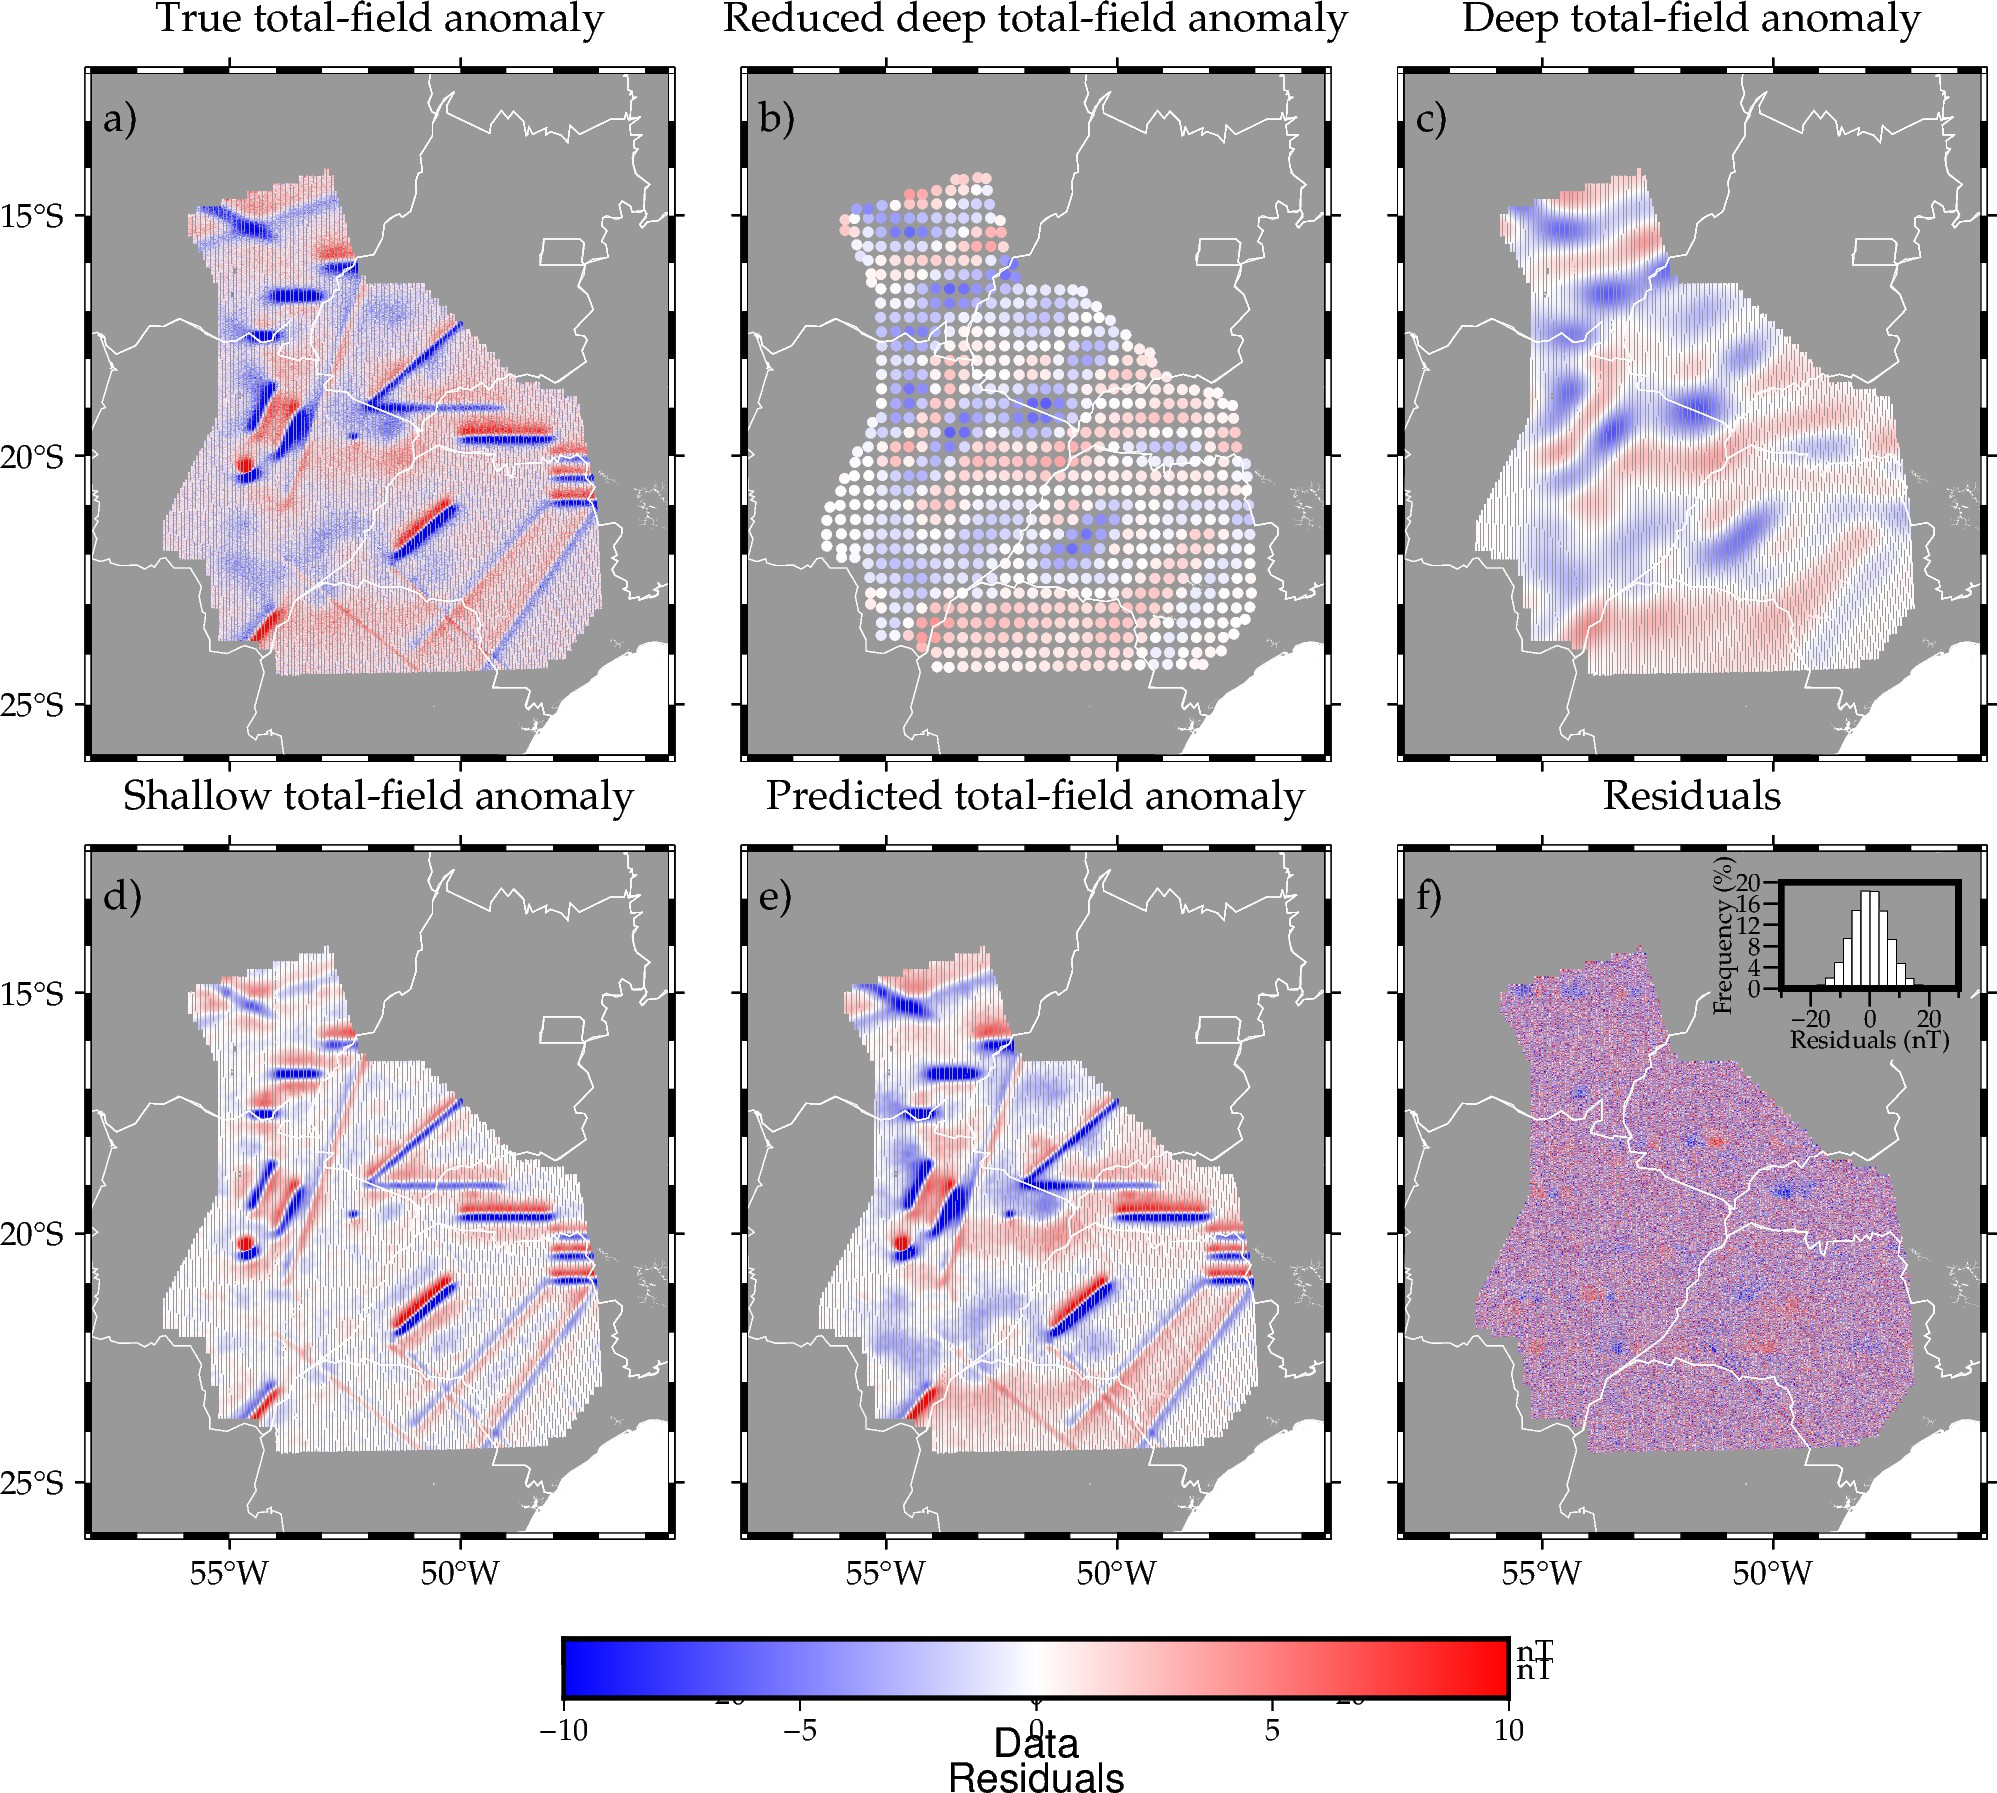
\includegraphics[width=1\linewidth]{figures/points-TFA-deep-shallow.jpeg}
    \caption{Illustration of the dual-layer decomposition process.
        \textbf{a)} True total-field anomaly.
        \textbf{b)} Deep total-field anomaly, capturing the long-wavelength
        regional field.
        \textbf{c)} Deep total-field anomaly, predicted on all data points.
        \textbf{d)} Shallow total-field anomaly, capturing the short-wavelength
        local anomalies.
        \textbf{e)} Predicted total-field anomaly.
        \textbf{f)} Residuals of the predicted model.}
    \label{fig_decomposition}
\end{figure}

\begin{figure}[!ht]
    \centering
    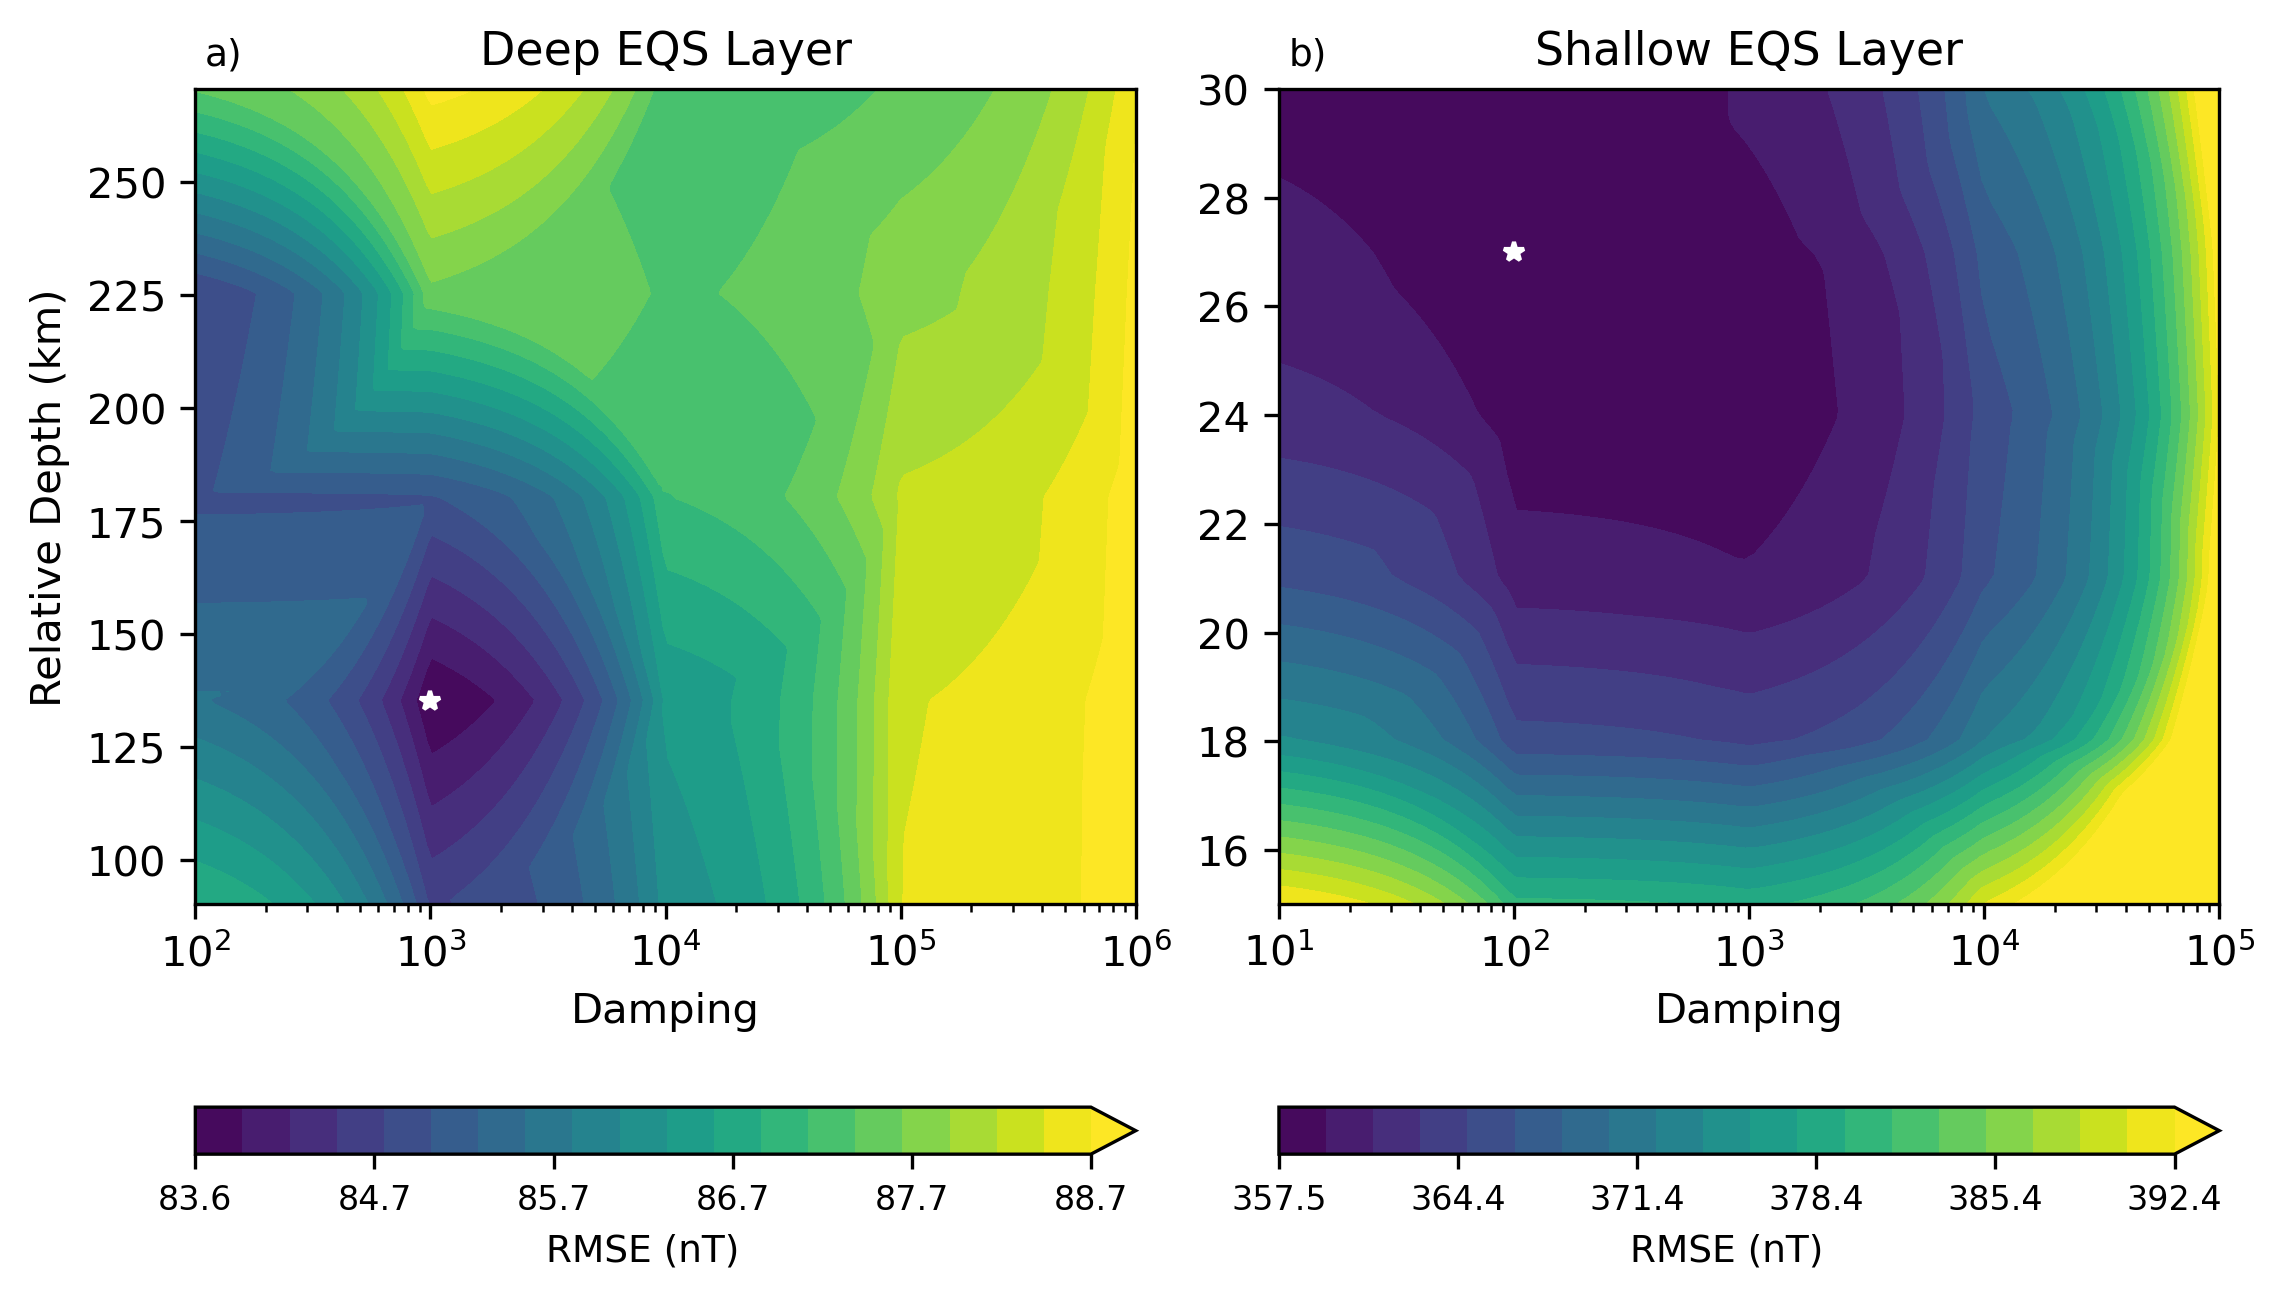
\includegraphics[width=1\linewidth]{figures/cv_synthetic.png}
    \caption{Block K-fold cross-validation results for the synthetic dataset.
    \textbf{a)} RMSE as a function of damping and relative depth for the deep
    equivalent sources layer, computed using the block-reduced dataset.
    \textbf{b)} RMSE obtained for the shallow layer using a cropped subset of
    the residual data. White stars indicate the selected optimal
    hyperparameter combinations corresponding to the minimum RMSE in each
    panel.}
    \label{fig_crossvalidation}
\end{figure}

\begin{figure}[!ht]
    \centering
    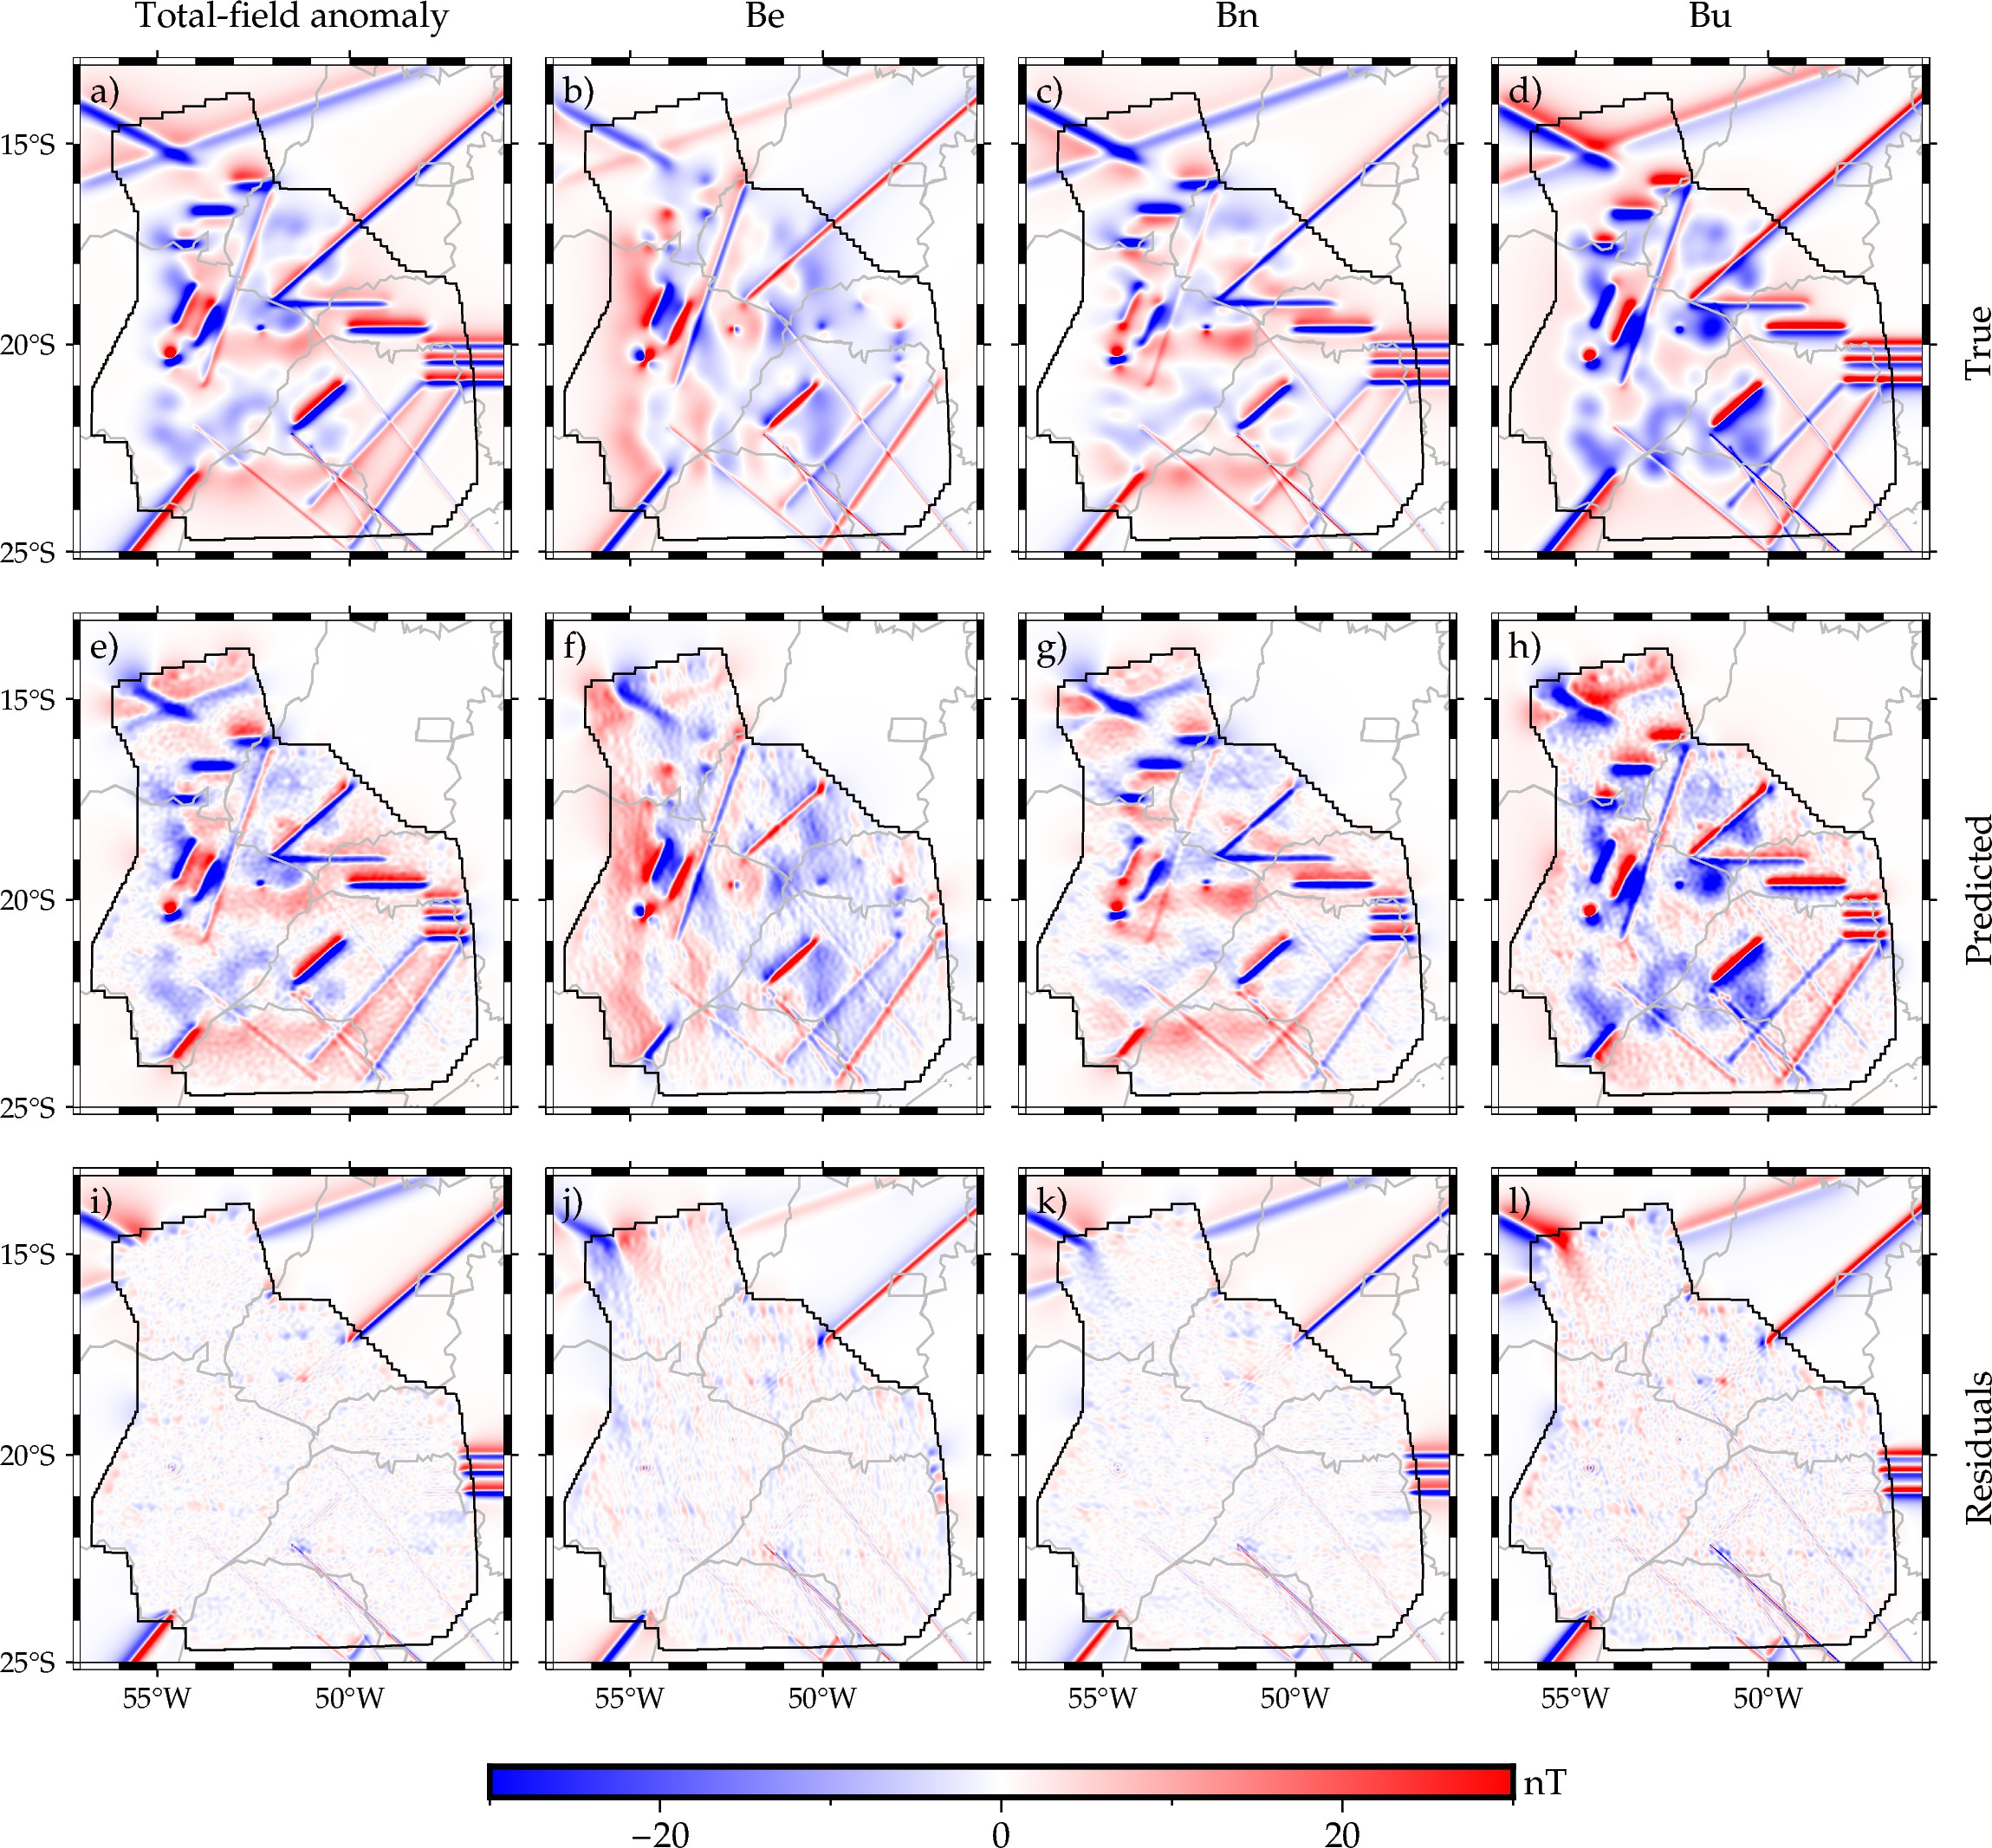
\includegraphics[width=1\linewidth]{figures/grided-TFA-B.jpeg}
    \caption{Gridded interpolation results for the total-field anomaly and its
        vector components (Be, Bn, Bu). The first row \textbf{(a-d)} shows the
        fields predicted (``Predicted'') by the dual-layer model. The second row
        \textbf{(e-h)} shows the true synthetic fields (``True'') for comparison.
        The third row \textbf{(i-l)} shows the final residuals (``Residuals"),
        corresponding to the difference between the true and predicted
        fields.}
    \label{fig_grid_results}
\end{figure}

To evaluate the performance and accuracy of the proposed methodology, we
applied it to a synthetic magnetic dataset designed to reproduce realistic
survey conditions. The model consists of multiple crustal sources with
different geometries, depths, and magnetizations, generating both regional
and local magnetic anomalies. The detailed configuration of the sources is
provided in the supplementary material \citep{archive}.

A complex regional magnetic field was generated using a deep distribution of
sources. Zero-mean Gaussian noise with a standard deviation corresponding to
5\% of the maximum absolute anomaly was added to the data to simulate
instrumental and environmental noise. The total field was computed assuming a
regional field with inclination $-25^{\circ}$ and declination $-20^{\circ}$,
consistent with the mean IGRF values in the study area.

To reproduce a realistic acquisition geometry, the synthetic field was
sampled along the flight lines of a public-domain aeromagnetic survey from the
Paraná Basin, Brazil. The original dataset, provided by the Agência Nacional
do Petróleo (ANP) and distributed through the CPRM/REATE portal
(\url{https://reate.cprm.gov.br/anp/TERRESTRE}), was preprocessed using a
block-reduction procedure. This operation resulted in $507,395$ observation
points, whose coordinates were used to generate the synthetic dataset. The
resulting total-field anomaly is shown in
Figure~\ref{fig_decomposition}a.

The deep layer was estimated from a block-reduced version of the synthetic
dataset in order to isolate the long-wavelength components of the magnetic
field. A block-reduction procedure based on the mean was applied using a
block size of $0.3^{\circ}$ in both latitudinal and longitudinal directions,
corresponding to approximately 33~km at the equator. This block size
represents a compromise between data compression and isolation of
regional-scale magnetic trends.
As a result, the original dataset containing 507,395 observations was reduced
to 795 data points, substantially decreasing the computational cost of the
deep-layer inversion while preserving the long-wavelength magnetic signal
(Figure~\ref{fig_decomposition}b).

The hyperparameters of the deep layer were selected through a block K-fold
cross-validation procedure applied to the block-reduced dataset. The tested
parameter space comprised five relative depths ranging from approximately
90~km to 270~km and five damping values varying from $10^{2}$ to $10^{6}$,
resulting in 25 parameter combinations. Spatial blocks of 1$^{\circ}$ (approximately
111~km) were used to avoid the spatial dependence between samples
in the training and testing sets during the cross-validation process.
The cross-validation results are shown in
Figure~\ref{fig_crossvalidation}a. The minimum RMSE was obtained for a relative
depth of approximately 135~km and a damping value of $10^{3}$. The error
surface exhibits a well-defined minimum around this configuration,
indicating limited sensitivity to moderate variations in the
hyperparameters and suggesting a stable regional-field solution.

Using the selected hyperparameters, the deep-layer inversion was performed
using the entire block-reduced dataset. The resulting model represents the
regional magnetic field and is shown in
Figure~\ref{fig_decomposition}b. The deep-layer was then used to predict the
total-field anomaly onto the full observation coordinates.
The residuals between the original data and the deep-layer prediction were
computed, these residuals constitute the input for the shallow-layer inversion.

The shallow layer was estimated using an iterative gradient-boosting
algorithm applied to the residuals of the deep layer. A window size of
2$^{\circ}$ (approximately 220~km) was adopted to limit the memory usage of the
inversion to the amount of RAM available.

Performing cross-validation on the entire residual dataset would be
computationally prohibitive due to the large number of observations.
However, since
the deep layer removes most of the long-wavelength signal, the remaining
residuals are dominated by local magnetic effects. Therefore, a
representative subset of the data was selected for hyperparameter tuning.
This subset was obtained by cropping the residual dataset to the region
bounded by longitudes $-54^{\circ}$ to $-52^{\circ}$ and latitudes
$-17^{\circ}$ to $-16^{\circ}$, resulting in 15,307 observation points. This
area contains a representative range of anomaly amplitudes and wavelengths,
preserving the spatial variability required for robust cross-validation.
A block K-fold cross-validation was then applied to this subset using spatial
blocks of 0.1$^\circ$ (approximately 12~km). This configuration ensures that neighboring
observations are not simultaneously used for training and validation,
reducing spatial bias. The tested hyperparameters comprised six relative
depths ranging from 15~km to 30~km and five damping values varying from $10^{1}$
to $10^{5}$, resulting in 30 parameter combinations.
The cross-validation results are shown in
Figure~\ref{fig_crossvalidation}b. The minimum RMSE was obtained for a relative
depth of approximately 27~km and a damping value of $10^{2}$. In contrast to
the deep layer, the RMSE surface exhibits a less well-defined minimum,
highlighting the decreased sensitivity of near-surface sources to parameter
variations.

The selected parameters were then applied to invert the full residual
dataset, producing the predicted total-field anomaly of the shallow-layer model shown in
Figure~\ref{fig_decomposition}d. The final residuals, obtained after combining
the deep and shallow predictions and subtracting them from the true data, are presented in
Figure~\ref{fig_decomposition}e. The low amplitude and spatially incoherent
distribution of the residuals indicate that the main magnetic features were
successfully modeled.

The estimated deep and shallow layers were then used to predict the magnetic field
onto a regular grid with a spatial resolution of 0.009$^\circ$ (approximately
1~km), constant height of
500~m, and dimensions of $1223 \times 1057$, totaling $3,878,133$ points. In
addition to the total-field anomaly, the eastward ($B_E$), northward ($B_N$),
and upward ($B_U$) components were also predicted.
The predicted grids are shown in Figure~\ref{fig_grid_results}a--d, together
with the true synthetic fields in Figure~\ref{fig_grid_results}e--h and the
difference between the true and predicted in Figure~\ref{fig_grid_results}i--l.
The difference maps exhibit low amplitudes and are largely free of coherent
spatial patterns within the main data coverage area, indicating an accurate
reconstruction of the observed magnetic field. Outside the core survey
region, moderately increased residuals reflect edge effects and reduced data
support near the survey boundaries. In regions dominated by high-frequency
anomalies associated with very shallow dike systems, localized residuals are
still observed, indicating that, despite the use of a dual-layer
parameterization, the extremely shallow nature of these sources poses
challenges for complete recovery.
Nevertheless, the proposed approach provides a robust alternative to
derivative-based transformations commonly used in magnetic data processing
and inversion, which are known to strongly amplify measurement noise and
acquisition-related artifacts. By estimating the full vector components
directly from total-field anomaly data through physically constrained
equivalent-source modeling, the method enables the use of physically
meaningful field attributes as inputs for subsequent inversion and
interpretation procedures.
This strategy allows the enhancement of short-wavelength features while
preserving numerical stability, avoiding the instability typically
introduced by high-order spatial derivatives. As a result, the predicted
field components constitute a reliable basis for further quantitative
analysis, particularly in high-noise environments where traditional
derivative operators often become unreliable.

The complete workflow, including the dual-layer inversion of 507,395
observations and prediction over 3,878,133 grid points, was completed in under
120~minutes on a personal computer equipped with an
Intel\textsuperscript{\textregistered} Core\textsuperscript{TM} i5-9300H CPU @
2.40~GHz (8 cores) and 16~GB of RAM, demonstrating the suitability of the
proposed methodology for processing large-scale magnetic datasets.

\section{Real Data Application}

\begin{figure}[tb]
    \centering
    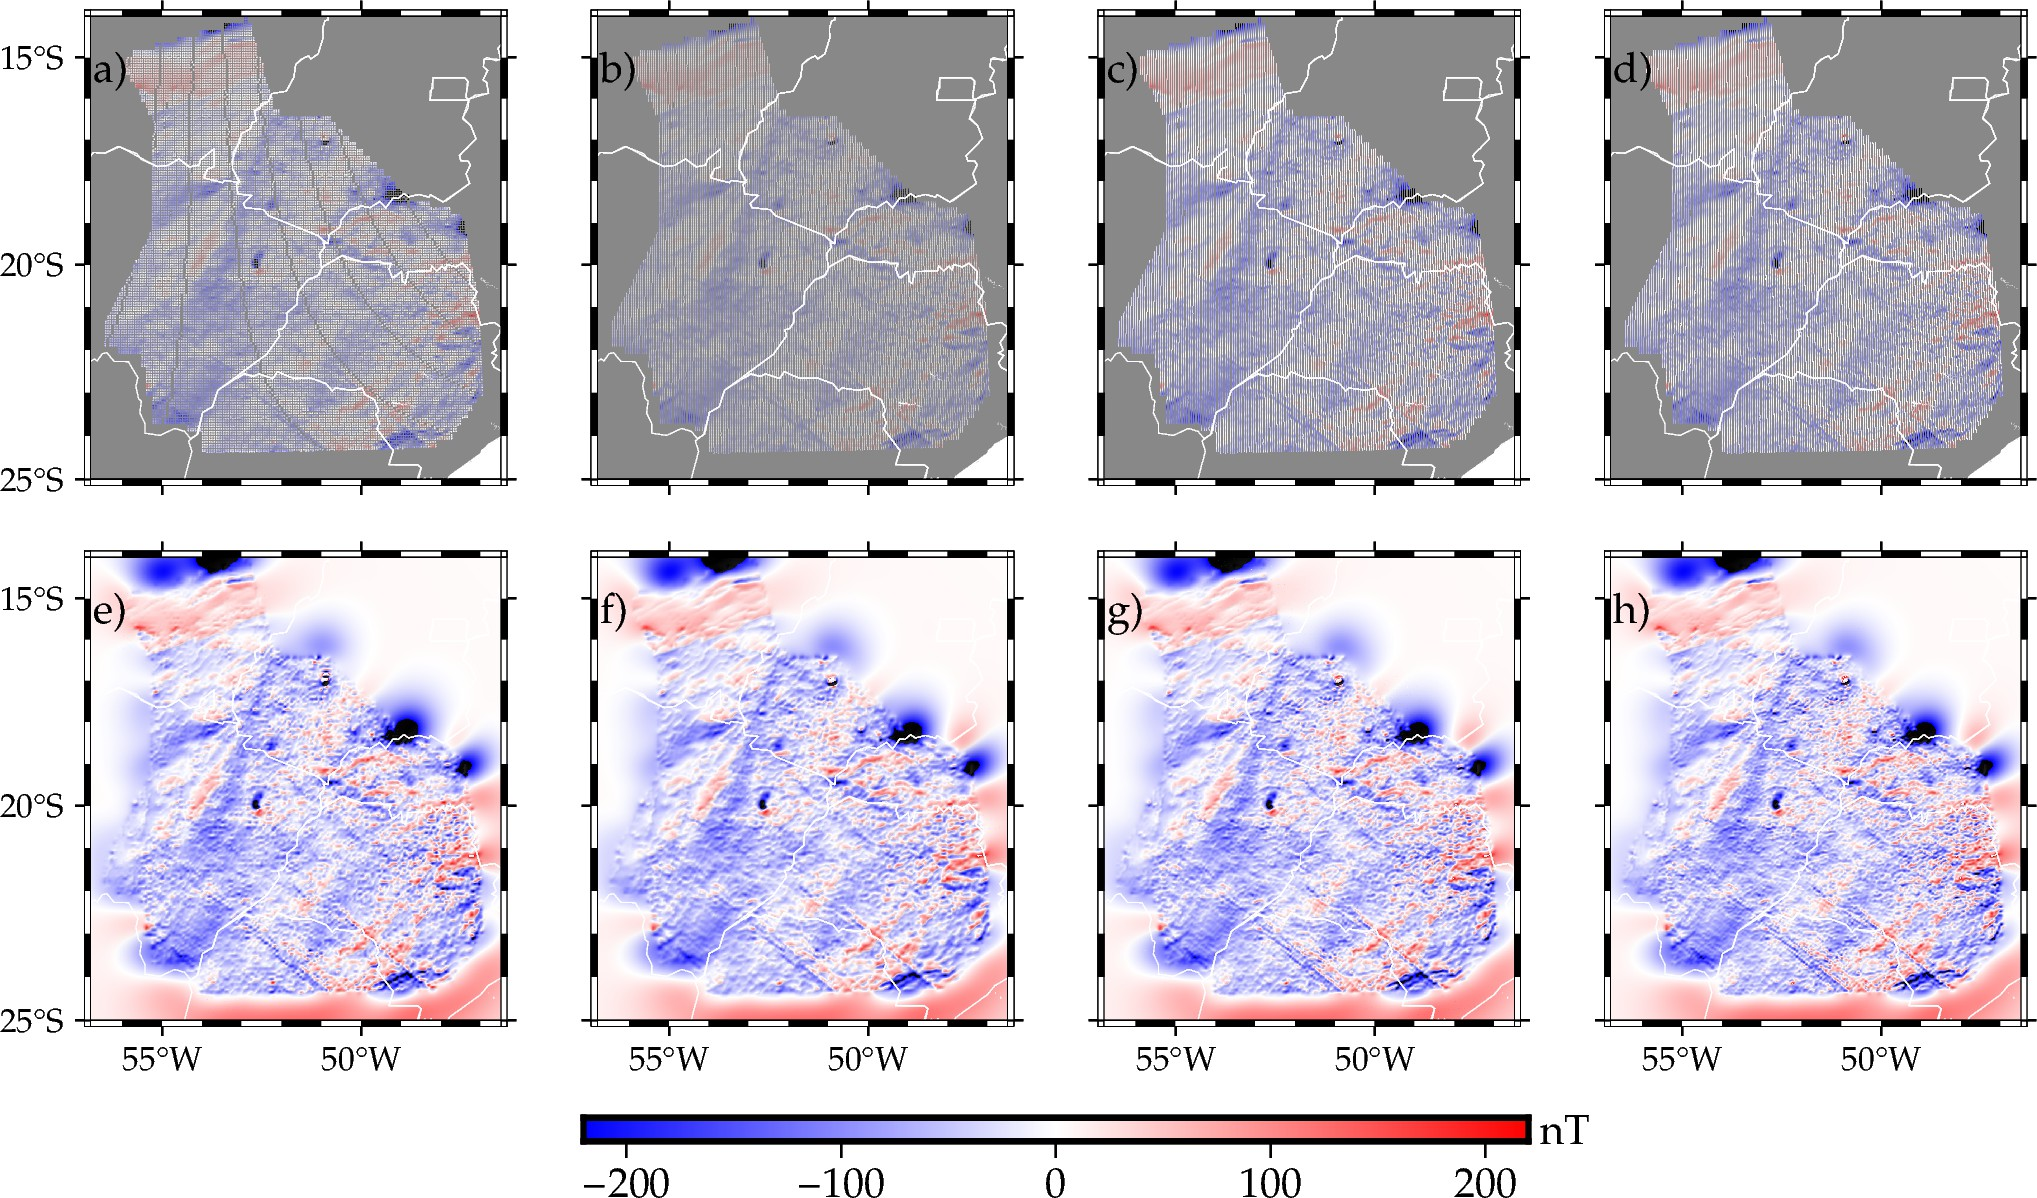
\includegraphics[width=1\linewidth]{figures/comparison-blockreduce.jpeg}
    \caption{Effect of varying block-mean size on the predicted total-field
    anomaly for the same region used in the Paraná Basin ANP data.
    \textbf{a--d)} Observed total-field anomaly gridded from different
    block-mean decimations. \textbf{e--h)} Predicted total-field anomaly
    using the spherical dual-layer gradient-boosted equivalent sources. The
    convergence of the predicted grids as the block size approaches the
    final grid resolution demonstrates the robustness of the method to
    sampling-density variations.}
    \label{fig_real_blockmean}
\end{figure}

\begin{figure}[!ht]
    \centering
    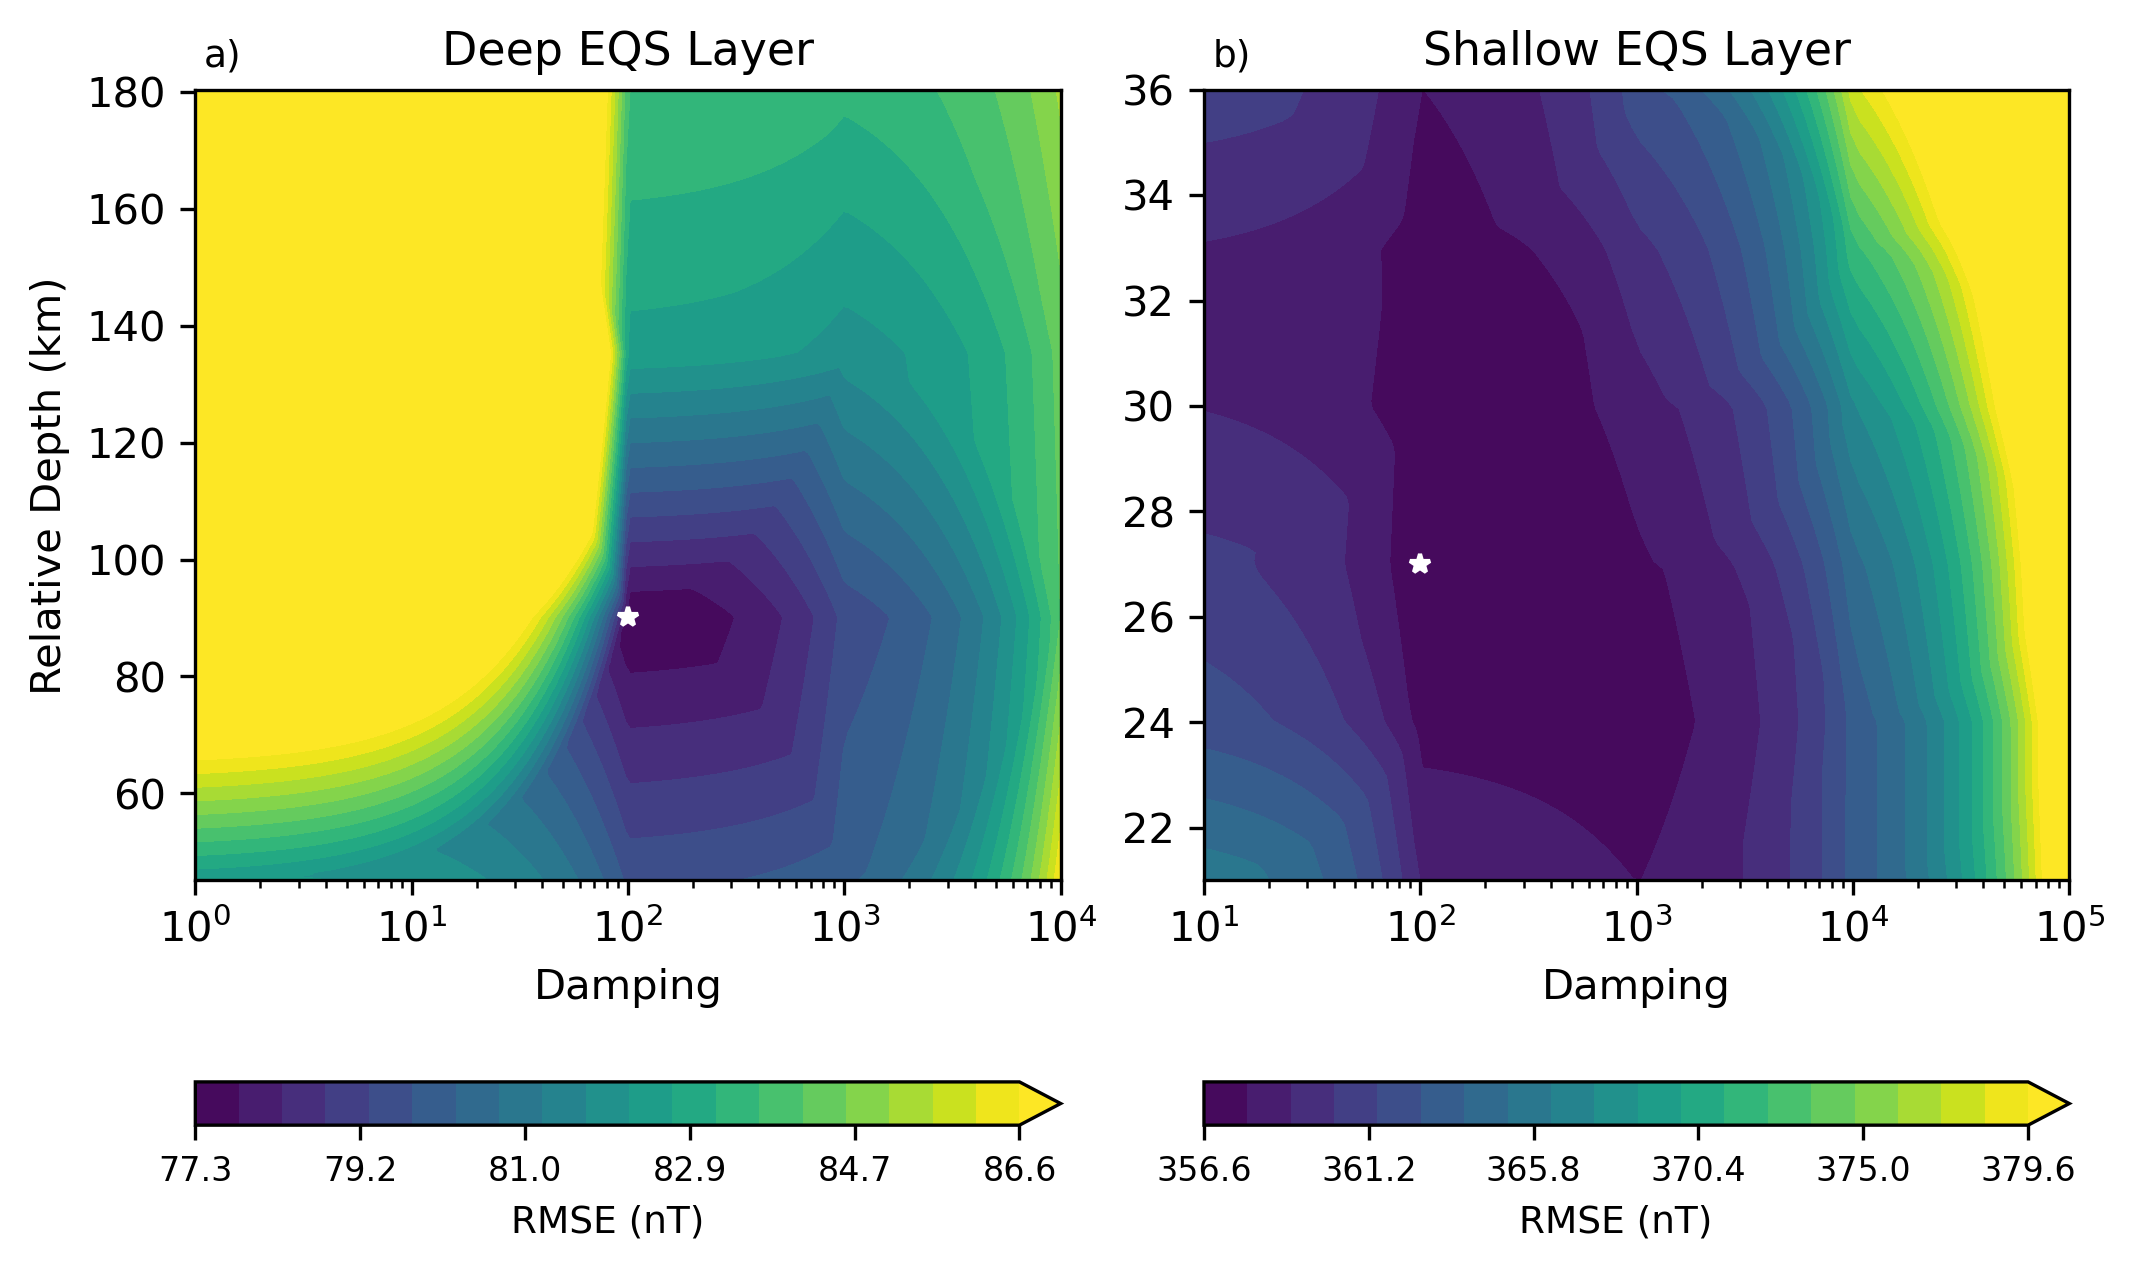
\includegraphics[width=1\linewidth]{figures/cv_real_00023.png}
    \caption{Block K-fold cross-validation results for the real dataset.
    \textbf{a)} RMSE as a function of damping and relative depth for the deep
    equivalent sources layer, computed using the block-reduced dataset.
    \textbf{b)} RMSE obtained for the shallow layer using a cropped subset of
    the residual data. White stars indicate the selected optimal
    hyperparameter combinations corresponding to the minimum RMSE in each
    panel.}
    \label{fig_real_crossvalidation}
\end{figure}

\begin{figure}[tb]
    \centering
    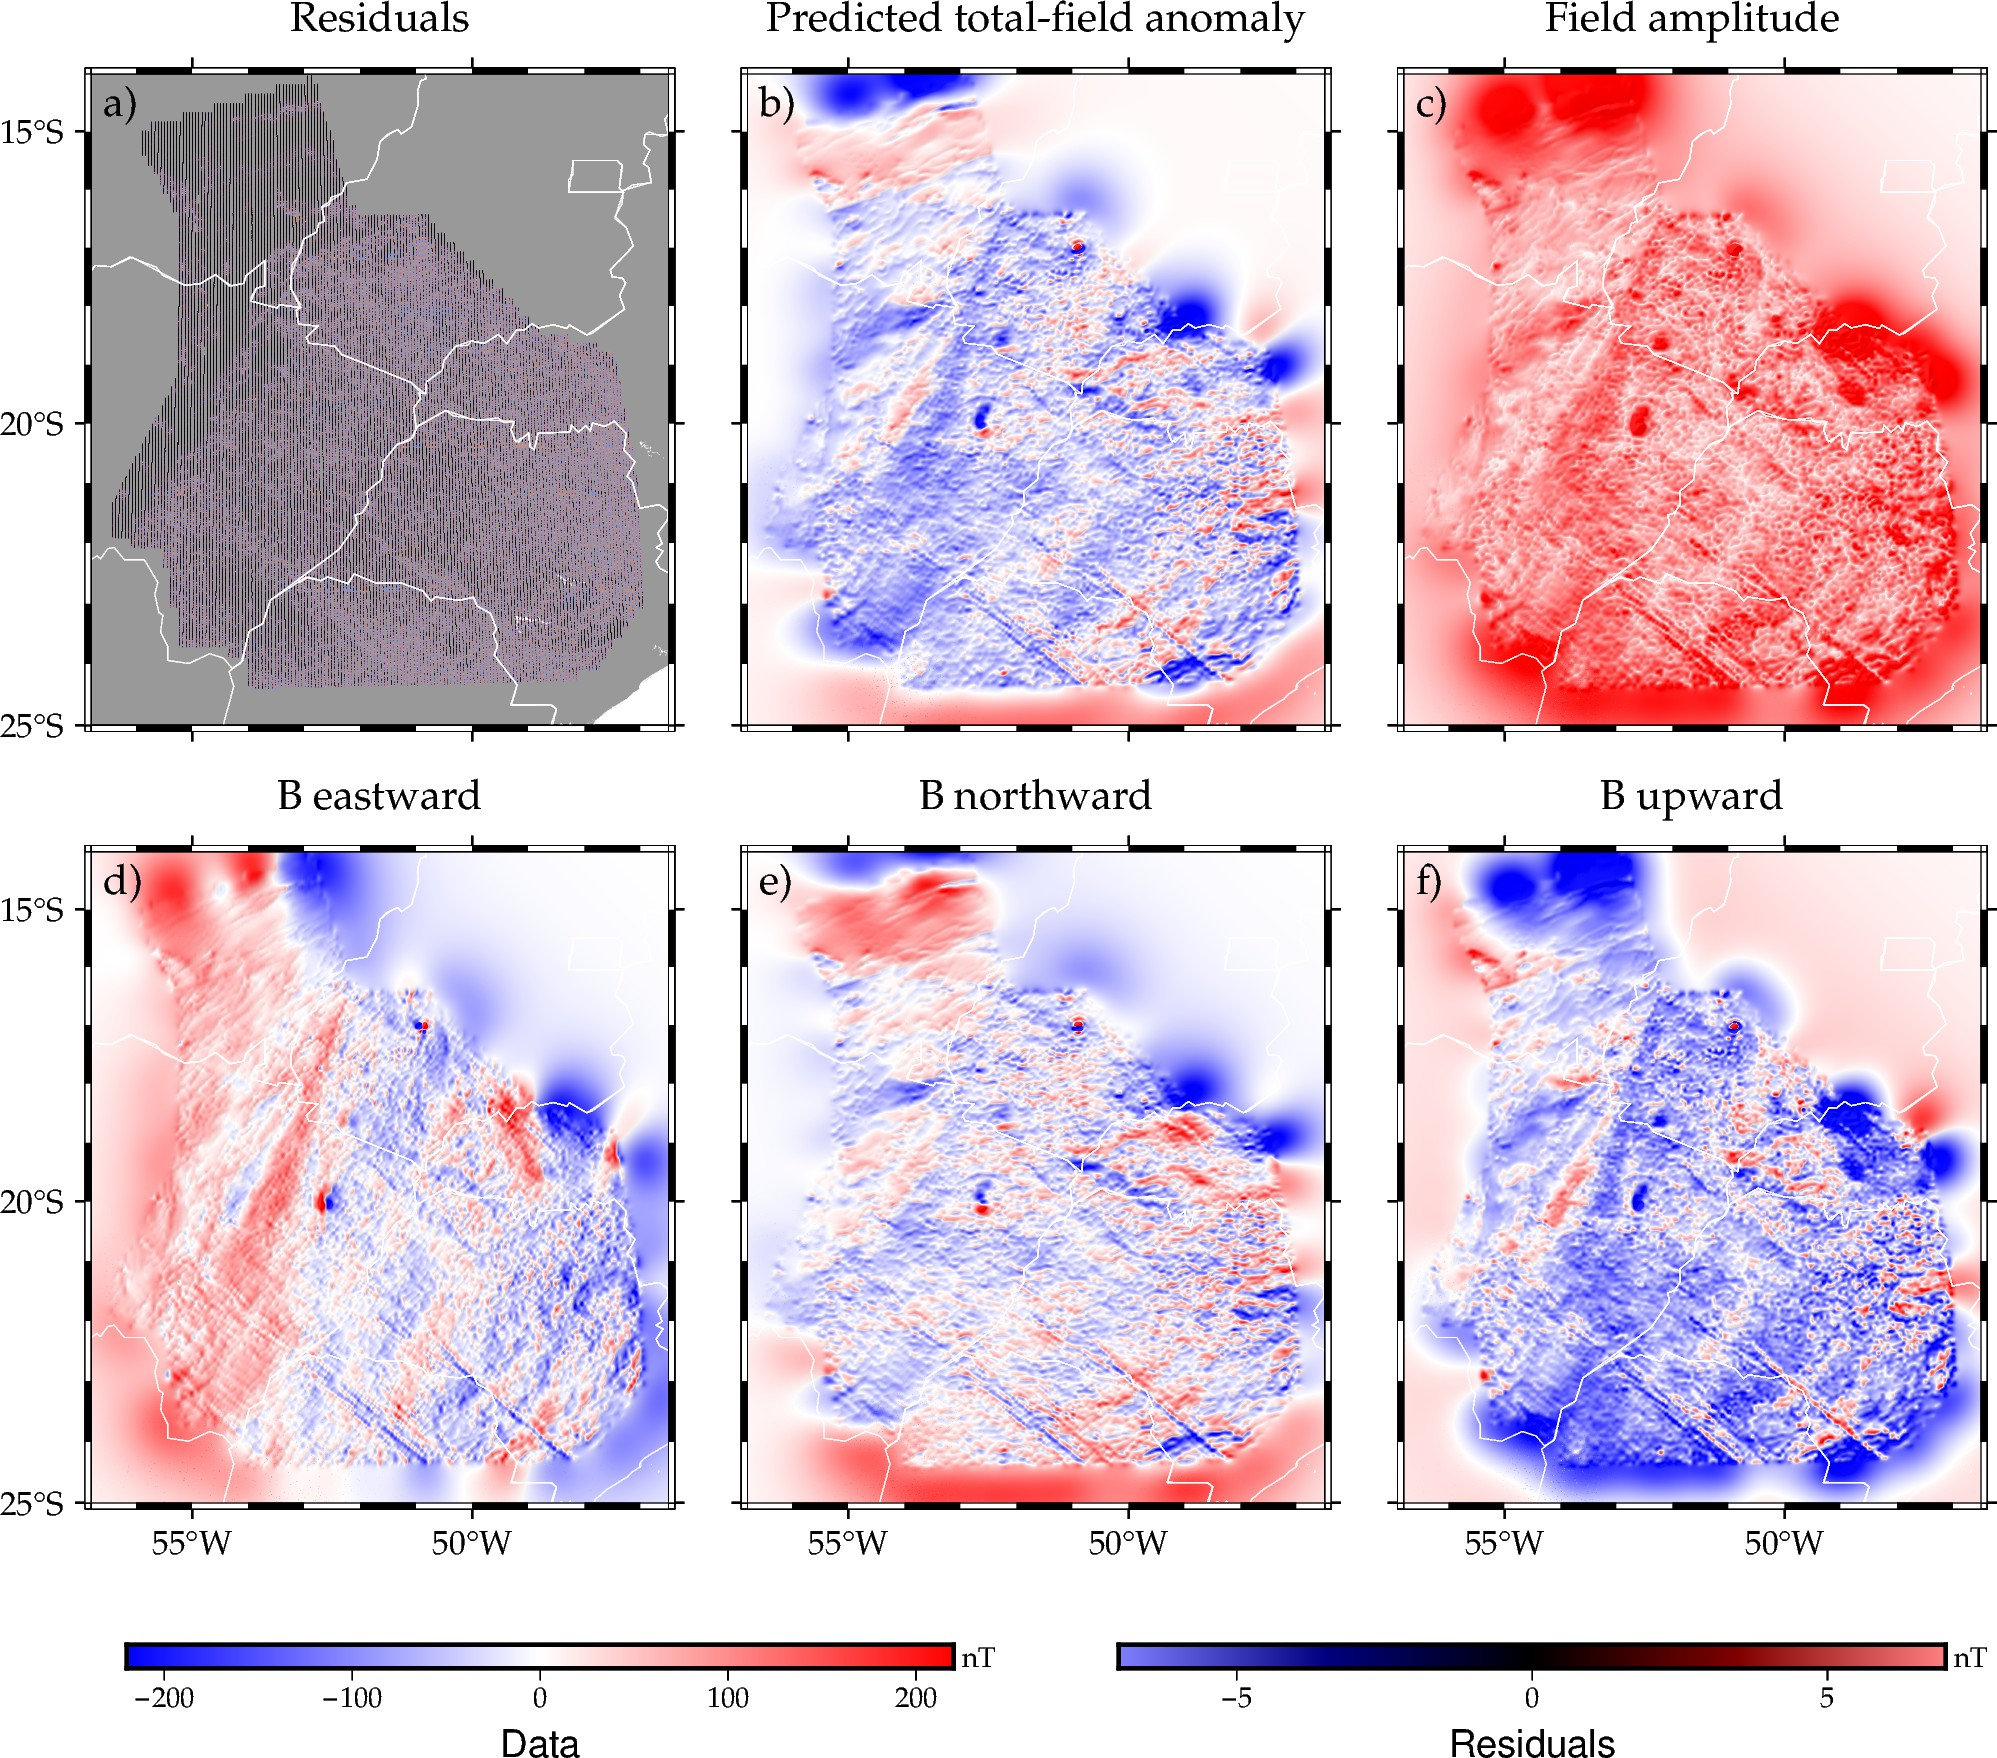
\includegraphics[width=1\linewidth]{figures/real-data-tfa-norm-bcomponents.jpeg}
    \caption{Predicted magnetic field for the Paraná Basin dataset.
    (\textbf{a}) Total-field anomaly. 
    (\textbf{b}) Amplitude of the anomalous magnetic field. (\textbf{d--f}) East, north, and upward
    components of the magnetic field. The
    smooth spatial behavior and coherence between components indicate the
    numerical stability of the proposed modeling approach.}
    \label{fig_real_components}
\end{figure}

To evaluate the performance of the proposed methodology under realistic
conditions, it was applied to airborne magnetic data acquired over the Paraná
Basin, Brazil.
The dataset, provided by the Agência Nacional do Petróleo (ANP;
\url{https://reate.cprm.gov.br/anp/TERRESTRE}),
covers latitudes from $-24.14^{\circ}$ to
$-14.14^{\circ}$ and longitudes from $-56.44^{\circ}$ to $-46.96^{\circ}$,
encompassing one of the largest sedimentary basins in South America.
Data acquisition was conducted along north--south flight lines spaced
approximately 6~km apart, with east--west control lines every 18~km, at an
average altitude of 1800~m. Horizontal and vertical positioning were obtained
using GPS, ensuring high positional accuracy. The dataset was originally
referenced to the SAD-69 datum and subsequently converted to WGS-84 using
official transformation parameters.
The original raw data were sampled at 100~Hz, which results in approximately
one data points every 8 cm.
This leads to an unnecessarily large dataset given the 6 km line spacing.
Hence, we decimated the data to 1~Hz by averaging consecutive groups of 100
samples along each flight line.
Numerical variables in the dataset were averaged, while categorical and identifier fields
were retained from the central record of each block. Records containing
corrupted or inconsistent values were discarded. This procedure preserves
along-line continuity while significantly reducing the dataset size. In
addition, tie lines were removed because they exhibited
inconsistent amplitude values, introducing spurious variations and systematic
distortions in the magnetic signal that could negatively affect the equivalent
sources modeling. After this preprocessing step, the resulting dataset with
1,636,695 observations is
illustrated in Figure~\ref{fig_real_blockmean}a.

Our target is to produce a regular grid at a constant height of 500~m and
a grid spacing of $0.0023^{\circ}$ (approximately 250~m).
The sampling density along flight lines of the 1~Hz data is larger than the
desired grid resolution.
Therefore, we investigated the sensitivity of the interpolation results to
different levels of data decimation.
The data were decimated using a block-mean operation with
two different block sizes, leading to three different configurations:
the complete dataset without decimation (Figure~\ref{fig_real_blockmean}a),
block size of $0.0023^{\circ}$ (approximately 250~m;
Figure~\ref{fig_real_blockmean}b), and
block size of $0.06^{\circ}$ (approximately 6.6~km; Figure~\ref{fig_real_blockmean}c). All
datasets were used to generate final grids with $0.0023^{\circ}$ resolution.
We used the same processing workflow for all datasets, which was the same as
the one applied to the synthetic data.
The deep layer was estimated from a block-mean version of each
dataset using a block size of $0.1^{\circ}$, corresponding to approximately
11~km, in order to isolate the long-wavelength signal.
For the cross-validation, we used
spatial blocks of $0.45^{\circ}$ (approximately 50~km) for the deep layer
and blocks of $0.18^{\circ}$ (approximately 20~km) for the shallow layer.
In addition, a window size of $1.5^{\circ}$ was used in the
gradient-boosting procedure of the shallow layer to control the amount of data
processed in each iteration, ensuring efficient memory usage and computational
stability.
The details of the cross-validation procedure for each dataset can be found in
the supplementary material \citep{archive}.
Using the same workflow for all three data decimation levels allows a direct
comparison of the outputs since source depth and damping regularization are
dependent on the input data geometry.

The predicted grids obtained from the different decimation
levels are shown in Figure~\ref{fig_real_blockmean}d--f.
The coarsest block-mean decimation ($0.06^{\circ}$) shown in
Figure~\ref{fig_real_blockmean}f resulted in the shortest
processing time (approximately 52~minutes).
However, it significantly attenuated short-wavelength magnetic anomalies,
compromising the recovery of near-surface sources and limiting its practical
applicability.
In contrast, the finest block-mean decimation ($0.0023^{\circ}$) shown in
Figure~\ref{fig_real_blockmean}e, corresponding to the target grid resolution,
required a processing time of approximately 10~hours and 48~minutes and
produced results that are nearly indistinguishable from those obtained using
the full dataset (Figure~\ref{fig_real_blockmean}d), which required
approximately 13~hours and 49~minutes.
Despite the higher computational cost, the $0.0023^{\circ}$ block-mean
decimation provides a roughly 20\% reduction in processing time relative to the
full dataset, while preserving the dominant short- and long-wavelength magnetic
features.

Based on this trade-off between computational efficiency and spectral
preservation, the dataset decimated with a block size of $0.0023^{\circ}$ was
selected for the subsequent analyses.
The hyperparameters of the deep layer were selected through a block K-fold
cross-validation procedure. The tested
parameter space comprised damping values of 1, 100, and 10,000 and source
depths of 70~km, 100~km, and 130~km, resulting in nine parameter combinations.
The cross-validation results are shown in
Figure~\ref{fig_real_crossvalidation}a. The minimum RMSE was obtained for a
relative depth of 100~km and a damping value of 100. The error surface exhibits
a well-defined minimum, indicating high sensitivity to moderate
hyperparameter variations.
The shallow layer was estimated using an iterative gradient-boosting
algorithm applied to the deep-layer residuals.
Due to the large number of observations, cross-validation on the entire
residual dataset would be computationally prohibitive. Therefore, a
representative subset was selected for hyperparameter tuning by cropping the
residual data to the region bounded by longitudes $-54^{\circ}$ to
$-50^{\circ}$ and latitudes $-18^{\circ}$ to $-16^{\circ}$.
A block K-fold cross-validation was applied to this subset.
The tested hyperparameters comprised damping
values of $10^{2}$, $10^{4}$, and $10^{6}$ and source depths of 6~km, 9~km, and
12~km, resulting in nine parameter combinations.
The cross-validation results are shown in
Figure~\ref{fig_real_crossvalidation}b. The minimum RMSE was obtained for the
optimal shallow-layer configuration of damping equal to $10^4$ and relative
source depth of 9~km.
The selected parameters were then applied to invert the full residual
dataset, producing the shallow-layer model. The final residuals
(Figure~\ref{fig_real_components}a), obtained
after combining the deep and shallow predictions, exhibit low amplitudes and
lack coherent spatial structures.

The estimated deep and shallow layers were subsequently used to predict the
magnetic field onto a regular grid with a spatial resolution of
$0.0023^{\circ}$ (approximately 250~m) and a
constant height of 500~m. In addition to the total-field anomaly
(Figure~\ref{fig_real_components}b), the amplitude (norm) of the magnetic field
(Figure~\ref{fig_real_components}c) and the eastward ($B_E$),
northward ($B_N$), and upward ($B_U$) components
(Figure~\ref{fig_real_components}d--f) were also computed.
The magnetic field amplitude centralizes the dipolar anomalies,
highlighting anomaly sources in a similar fashion to the total gradient
amplitude.
The $B_E$ component
emphasizes predominantly north--south-oriented features, whereas the $B_N$
component enhances east--west-trending structures. The $B_U$ component also
exhibits mostly centered anomalies, consistent with the distribution observed
in the total-field anomaly and amplitude maps. Together, these results confirm the ability
of the proposed methodology to recover multiple components of the anomalous
magnetic field from observations of the total-field anomaly.

%%%%%%%%%%%%%%%%%%%%%%%%%%%%%%%%%%%%%%%%%%%%%%%%%%%%%%%%%%%%%%%%%%%%%%%%%%%%%%%
\chapter{Conclusions}

This study presented and systematically validated a spherical equivalent
sources framework for large-scale magnetic data processing, interpolation, and
transformation. The proposed methodology integrates dual-layer equivalent
sources modeling \citep{Uppal2025,Li2020}, gradient-boosting
\citep{Soler2021}, and spatial cross-validation into a unified and
computationally efficient workflow.
Our equivalent sources formulation can work with data in both spherical and
geodetic coordinate systems.

The synthetic data experiments demonstrated that the dual-layer configuration
provides a robust mechanism for separating long- and short-wavelength
magnetic components under realistic acquisition geometries and noise
conditions. The adopted block-reduction strategy for the deep layer reduced
the original dataset from more than 500,000 observations to fewer than 1,000
points while preserving the dominant regional signal. This reduction enabled
efficient hyperparameter tuning and inversion without compromising spectral
fidelity.
Cross-validation results obtained from the synthetic dataset showed a
well-defined minimum for the deep layer, indicating a stable solution.
The cross-validation of the shallow layer
exhibited a less well-defined minimum, reflecting the decreased sensitivity of
near-surface sources to depth and regularization. These results highlight the
importance of independent parameter tuning and justify the adoption of separate
optimization strategies for regional and local components.
Moreover, our synthetic data results show that our spherical dual-layer method
is able to accurately recover the magnetic field components from the
total-field anomaly observations.
This was shown to be theoretically possible through the use of Fourier
transform by \citet{Lima2009} and through the use of equivalent sources by
\citet{Li2020}.
Here, we demonstrate that this can also be achieved in a spherical or geodetic
reference frame through the use of equivalent sources.

The application to real airborne magnetic data from the Paraná Basin confirmed
the scalability and robustness of the proposed workflow under realistic
conditions, including heterogeneous sampling density, acquisition artifacts,
and large data volumes (upward of 1.5 million data points). A detailed analysis
of different spatial decimation strategies demonstrated that decimation using
coarse block sizes (of the order of the line spacing), although computationally
efficient, leads to significant attenuation of short-wavelength anomalies and
compromises the recovery of near-surface sources. Conversely, data decimation
using a block size that is compatible with the final grid resolution preserved
the amplitude of short-wavelength anomalies and resulted in a grid that is
largely indistinguishable from the one produced with the full dataset.
Moreover, the processing time for the reduced dataset was approximately 20\%
smaller than for the full dataset. Therefore, we recommend always decimating
the input data using a block mean operation with block size equal to the
desired grid spacing \citep{Smith1990}.

The availability of vector components provides some advantages over traditional
derivative-based interpretation techniques. Magnetic derivatives are inherently
sensitive to noise, interpolation artifacts, and uneven data coverage,
particularly in continental-scale surveys. In contrast, the
equivalent-source-based predicted field components and amplitude produces
smooth, physically constrained fields that retain geological meaning while
avoiding noise amplification.
The anomalous field amplitude is particularly useful for interpretation and
geometry inversion workflows.
As demonstrated by \citet{HidalgoGato2021},
the inversion of basement relief from the amplitude of the magnetic field
is only
weakly dependent on the often unknown magnetization direction. This characteristic
allows reliable structural characterization even in the presence of
remanent magnetization and limited prior information. Consequently, the
framework proposed here offers a solid foundation for subsequent structural
mapping, susceptibility inversion, and integrated geophysical modeling.

Overall, the results indicate that the spherical dual-layer
gradient-boosted equivalent sources method constitutes a flexible, scalable,
and physically consistent solution for magnetic data processing. The
framework is capable of handling very large datasets while preserving
short- and long-wavelength of the magnetic field and maintaining manageable computational
requirements.
The method proposed here is able to handle millions of
data points in a modest computer in the timescale of hours.
However, the spherical calculations are significantly slower than their
Cartesian counterparts.
Thus, the current formulation will likely struggle to process larger
compilations involving multiple surveys and tens to hundreds of millions of
data points without access to significant computational resources.
Further optimization of the equivalent sources methods would be required to
make it feasible to use our method to generate a consistent and integrated
model for continental scale data compilations.

\bibliographystyle{apalike-doi}
\bibliography{references}

\end{document}
